\documentclass[a4paper,11pt]{scrartcl}

\usepackage[utf8]{inputenc}
\usepackage[ngerman]{babel}
\usepackage[T1]{fontenc}
\usepackage{amsmath}
\usepackage{graphicx}
\usepackage{tabularx}
\usepackage[a4paper, left=2cm, right=2cm, top=2.8cm, bottom=2.8cm]{geometry}
\usepackage{tikz}   
\usepackage[scaled]{helvet}
\usepackage{tabto} 
\usepackage{fancyhdr}
\usepackage{multirow}
\usepackage{pdfpages}

\renewcommand*{\familydefault}{\sfdefault}

\pagestyle{fancy}

\setkomafont{section}{\huge}
\setkomafont{subsection}{\Large}


\lhead{Maximilian Hoffmann}
\chead{Betrieblicher Auftrag \\ \textbf{Kabeltester}}
\rhead{
\includegraphics[width=3cm]{Bilder/BMK_LOGO.png}}


\title{Abschlussprojekt \\ Kabeltester}
\author{Maximilian Hoffmann}
\date{\today}

\begin{document}

\maketitle
\begin{center}
   \includegraphics[width=15cm]{Bilder/Kabeltester.jpg}
\end{center}

\vspace{1,5cm}

\renewcommand{\arraystretch}{2}
\begin{center}
\begin{tabular}[h] {c|c}
\textbf{Auftragnehmer} 		& 	\textbf{Auftraggeber} 		\\
Maximilian Hoffmann			& 	Robert Schulz				\\
BMK Group GmbH Co.KG		&	BMK Group GmbH Co.KG		\\
Werner-von-Siemens-Straße 6	&	Werner-von-Siemens-Straße 6 \\
Entwicklung Labor			& 	Entwicklung		
\end{tabular}
\renewcommand{\arraystretch}{1}
\end{center}


\newpage

\vspace{2cm}

\begin{center}
\begin{Huge}
\textbf{Änderung}
\end{Huge}
\end{center}
Das Lastenheft, welches bei der Projektgenehmigung mit eingereicht wurde, weißt einen Fehler auf. 
\\
Es war zu jedem Zeitpunkt zwischen mir und meinem Auftraggeber klar, dass von meiner Seite aus, ein Prototyp entwickelt werden soll. Eine Lebenszeitberechnung für ein noch nicht fertiggestelltes Produkt ist daher nicht sinnvoll.
\\
In der ersten Version des Lastenheftes, wurde dieses Detail leider nicht schriftlich festgehalten. Dies hat sich in meiner nun folgenden Dokumentation geändert.



\vspace{5cm}

\begin{Huge}
\begin{center}
\textbf{Wichtige Anmerkung}
\end{center}
\end{Huge}
Bei der vorliegenden Dokumentation handelt es sich um eine umfassende Dokumentation zu meinem Projekt. 
\\
Diese beinhaltet in kombinierter Form die Dokumentation für die IHK und meinem Auftraggeber.
\\
Die mit transparenter blauer Farbe markierten Abschnitte sind für die IHK-Abschlussprüfung relevant. 
\\
Die mit transparenter roter Farbe markierten Abschnitte sind die nicht für die IHK relevanten Dokumentationsteile. Sie sind von meinem Auftraggeber gefordert und sollen dem Prüfungsausschuss nur zum Verständnis dienen.




\newpage

\tableofcontents
\newpage



\section{Klärung der Begrifflichkeiten}

\subsection{BMK-IoT Modul}
Das „BMK-IoT Modul“ ist ein Design In Modul. Eine bereits entwickelte Hardwaregrundlage mit Mikrocontroller, WLAN-Chip, eMMC und Standard-Schnittstellen, sowie fertigen Softwaregrundlagen im Bereich der Embedded Security, RTOS und Cloud ermöglichen der BMK-Entwicklung kundenspezifische Projekte schneller und einheitlicher zu realisieren.
Die dafür benötigte Hardware findet auf einer kleinen Platine mit BGA-Sockel Platz. 

\begin{center}
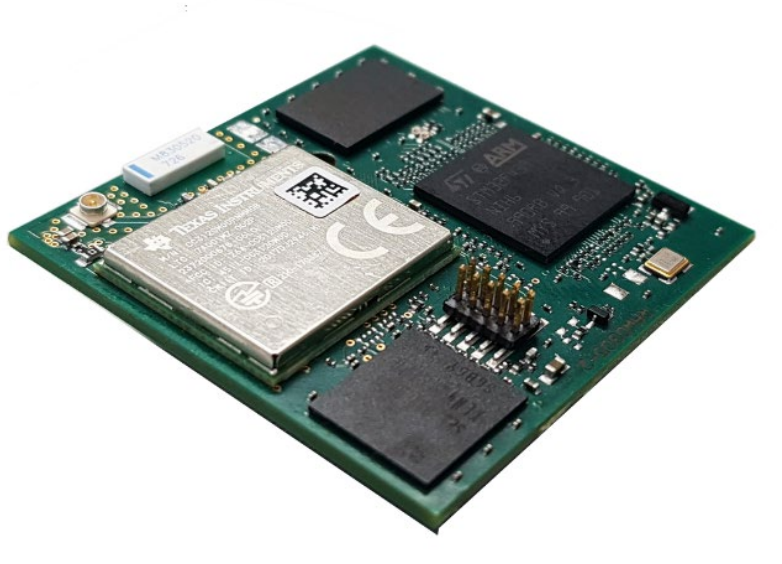
\includegraphics[width=10cm]{Bilder/BMK-IOT-MODUL.png}
\end{center}

\subsection{eMMC}
eMMC = embedded MultiMediaCard.
\\
Ein \glqq eMMC \grqq{} ist eine Variante eines Speicherkarten Standards. Durch seine preiswerte kompakte Größe wird diese Art häufig in mobile Endgeräte verbaut. Die verwendete Technologie ist die eines Flash-Speichers . Flash-Speicher und Flash-Controller werden auf dem selben Silizium-Chip integriert. Dabei sind Übertragungsraten bis zu 400MB/s möglich. eMMC's werden häufig direkt verlötet und sind deshalb ein Teil eines \glqq embedded System \grqq{}.


\subsection{RTOS}
RTOS = Real Time Operating System
\\
Ein \glqq Real Time Operating System \grqq{} besitzt die grundlegende Aufgabe, zu entscheiden welcher Task (Programmteil) wann ausgeführt wird. Für den Anwender, soll es dabei so aussehen, als ob die Anwendungen gleichzeitig abgearbeitet werden. In der Realität werden den Task's verschiedene Priorisierungen zugewiesen. Dadurch kann der Prozess-Scheduler entscheiden, welche Task wann und vor welchen anderen Task's abgearbeitet wird. 
\\
Nicht nur im Bereich des \glqq Event Handlings \grqq{} ist ein RTOS sehr wichtig, sondern auch im Bereich des Speicherzugriffes bieten sich RTOS-spezifische Funtionen an. Kommt es z.B. zu einem gleichzeitigen Speicherzugriff zweier Prozessorkerne, so kann es zu fatalen Fehlern kommen. Eine Priorisierung ist hier ebanfalls sehr wichtig.

\newpage
\subsection{BGA}
BGA = Ball Grid Array
\\
Unter \glqq BGA\grqq versteht man eine Art der Gehäuseform, wobei die Anschlüsse für die SMD-Bestückung auf der Unterseite des Bauteiles liegen. Kleine Lötperlen auf der Unterseite, können dabei durch einen Reflow-Prozess mit der Platine verlötet werden. Diese Technologie lässt dabei eine große Menge an Pin's auf einem kleinen Chip zu. 


\subsection{Pig-Tail}
Um bei hohen Frequenzen mit einem Oszilloskop bessere Messergebnisse zu erhalten, ist es oft hilfreich, ein Pig-Tail zu verwenden. Diese können oft beim Hersteller gekauft oder mit Silberdraht selbst gewickelt werden. 
\\
Das Messergebnis verbessert sich durch die niedrigere Induktivität der Masseleitung. Das über bzw. unterschingen des Messsignales verringert sich dadurch sichtbar. 


\begin{center}

\includegraphics[width=10cm]{Bilder/PigTail.jpg}


\end{center}


\begin{figure}[htb]
    \centering
    \begin{minipage}[t]{0.45\linewidth}
        \centering
        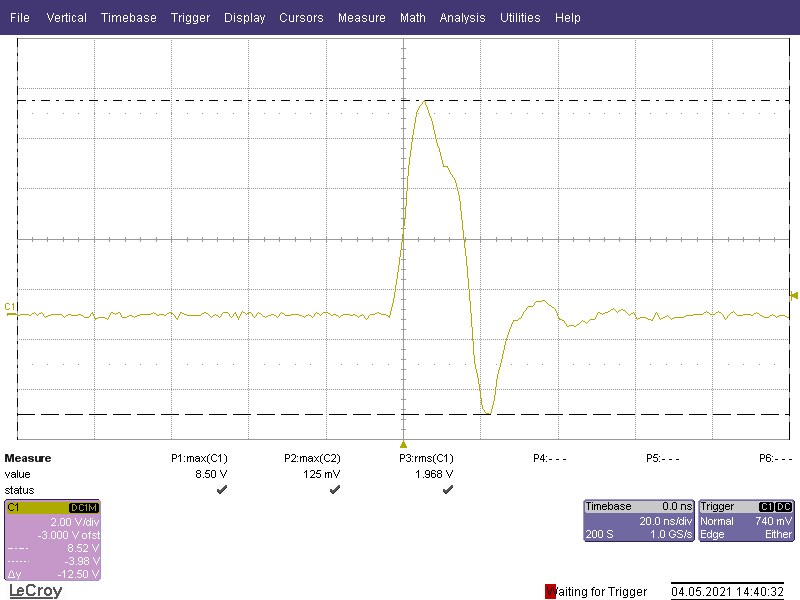
\includegraphics[width=8cm]{Bilder/TP19-ohne-PigTail.png}
        \caption{Signal ohne Pig-Tail}
    \end{minipage}% <- sonst wird hier ein Leerzeichen eingefügt
    \hfill
    \begin{minipage}[t]{0.45\linewidth}
        \centering
        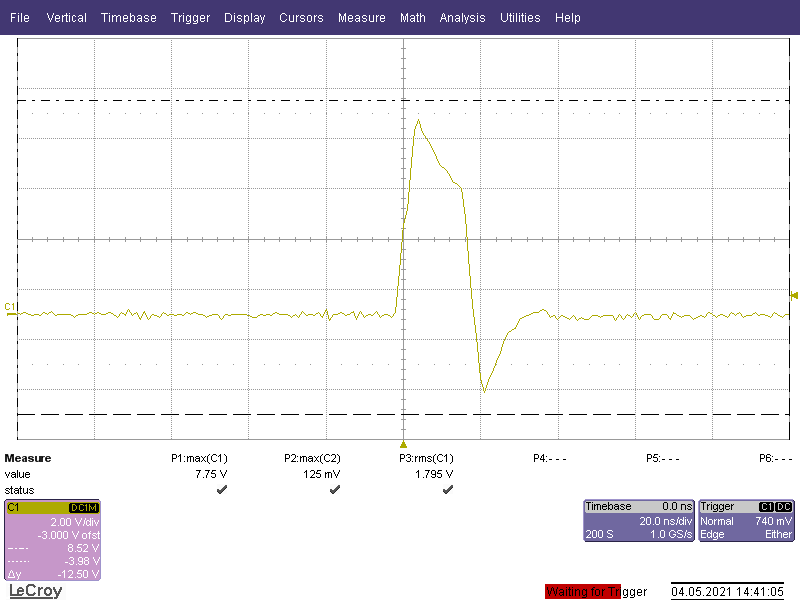
\includegraphics[width=8cm]{Bilder/TP19-mit-PigTail.png}
        \caption{Signal mit Pig-Tail}
    \end{minipage}
\end{figure}

\newpage


%%%%%%%%%%%%%%%%%%%%%%%%%%%%%%%%%%%%%%%%%%%%%%%%%%%%%%%%%%%%%%%%%%%%%%%%%%%%%%%%%%%%%%%%%%%%%%%%%%%%%%%%%%%%%%%%%%%%%%%%%%%%%%%%%%%%%%%%%%%%%%%																																			 %
%														Ausgangssituation																     	 %
%																																		     %
%%%%%%%%%%%%%%%%%%%%%%%%%%%%%%%%%%%%%%%%%%%%%%%%%%%%%%%%%%%%%%%%%%%%%%%%%%%%%%%%%%%%%%%%%%%%%%%%%%%%%%%%%%%%%%%%%%%%%%%%%%%%%%%%%%%%%%%%%%%%%%


\section{Ausgangssituation}

%%%%%%%%%%%%%%%%%%%%%%%%%%%%%%%%%%%%%%%%%%%%%%%%%%%%%%%%%%%%%%%%%%%%%%%%%%%%%%%
%																			  %
%								BMK-Entwicklung								  %
%																			  %
%%%%%%%%%%%%%%%%%%%%%%%%%%%%%%%%%%%%%%%%%%%%%%%%%%%%%%%%%%%%%%%%%%%%%%%%%%%%%%%

\subsection{BMK-Entwicklung}
Neben der Tätigkeit als EMS-Dienstleister (Electronics Manufacturing Services), bietet die \glqq BMK Group GmbH  Co. KG \grqq{} auch eine kundenspezifische Elektronikentwicklung an. Die Entwicklung von Software, Hardware und Layout erfolgt unter dem Namen\glqq BMK-Entwicklung \grqq{} . 
Zu meinen Aufgaben in der BMK-Entwicklung gehört es, den Hardwareentwicklern und Softwareentwicklern bei ihren täglichen Aufgaben bei Seite zu stehen. 

%%%%%%%%%%%%%%%%%%%%%%%%%%%%%%%%%%%%%%%%%%%%%%%%%%%%%%%%%%%%%%%%%%%%%%%%%%%%%%%
%																			  %
%								BMK-Testentwicklung							  %
%																			  %
%%%%%%%%%%%%%%%%%%%%%%%%%%%%%%%%%%%%%%%%%%%%%%%%%%%%%%%%%%%%%%%%%%%%%%%%%%%%%%%

\subsection{BMK-Testentwicklung / Testentwicklungslabor}
Eine weitere Dienstleistung der \glqq BMK Group \grqq{} ist die \glqq Testentwicklung \grqq{}. Im Haus gefertigte Baugruppen, durchlaufen während des Fertigungsprozesses verschiedene Testschritte. Die Entwicklung von Testadaptern, wird auf Kundenwunsch von der BMK-Testentwicklung übernommen. Standardisierte Testverfahren hierbei sind: ICT-Test (Integrated Circuit Test), FKT-Test (Funktionstest) und Boundary-Scan. Der Aufbau eines Testadapters wird dabei durch das Testentwicklungslabor übernommen. 

%%%%%%%%%%%%%%%%%%%%%%%%%%%%%%%%%%%%%%%%%%%%%%%%%%%%%%%%%%%%%%%%%%%%%%%%%%%%%%%
%																			  %
%								Testverfahren Akutell						  %
%																			  %
%%%%%%%%%%%%%%%%%%%%%%%%%%%%%%%%%%%%%%%%%%%%%%%%%%%%%%%%%%%%%%%%%%%%%%%%%%%%%%%

\subsection{Aktuelles Testverfahren für Programmierkabel sowie Flachbandkabel}
Das derzeitige Testverfahren für Programmierkabel in der Softwareentwicklung erfolgt nach dem\glqq Try and Error – Prinzip \grqq{} . Kann der Softwareentwickler keine Verbindung mit den gefertigten Programmierkabeln zwischen Controller und Programer aufbauen, so muss das Problem zeitaufwendig analysiert werden.
\\
Ist ein Testadapter des Testentwicklungslabors fertiggestellt, so wird dieser abschließend durch einen anderen Mitarbeiter überprüft. Dabei wird jede einzelne Leitung mit Hilfe eines Multimeters anhand des Schaltplanes überprüft. Flachbandkabel, welche Adapterkassette und Nadelbett miteinander verbinden, mussten sich bisher keinen Prüfungsprozess unterziehen. 


\newpage
\section{Auftragsplanung}

Ursprünglich war das Einsatzumfeld meines betrieblichen Auftrages für die BMK-Entwicklung vorgesehen. Während der Erstellung eines Lastenheftes stellte sich heraus, dass auch das Testentwicklungslobor an einem solchen Prüfgerät Interesse hat. 



\subsection{Auftragsziel}

Ziel des betrieblichen Auftrages ist die Entwicklung eines Prüfkonzeptes, sowie den dazugehörigen Prototypen einer Prüfvorrichtung zum Prüfen verschiedener konfektionierter Kabel. Das Prüfkonzept dieses Prototyps soll im Endzustand eine Prüfung verschiedener BMK-Standard-Programmierkabeln und Flachbandkabeln übernehmen. 
In Zukunft soll dadurch eine Menge Zeit bei der Fehlersuche eingespart werden und die Übergabe von fehlerhaften Programmierkabeln an einen Softwareentwickler ausgeschlossen werden.
Das Prüfgerät soll nach dem „stand alone“ -Prinzip funktionieren und für den Anwender einfach zu bedienen sein.


\subsection{Anforderungen}

Durch Rücksprache mit dem Auftraggeber wurden folgende Details ausgearbeitet. Diese wurden außerdem in einem offiziellen Pflichtenheft festgehalten. 

\begin{itemize}
	\item{Die extern angelegte Versorgungsspannung (Akku oder Batterie) soll möglichst verlustfrei auf einen 5V TTL-Pegel gewandelt werden. }

	\item{Die Leitungen sollen auf Durchgängigkeit, sowie auf Kurzschlüsse untereinander geprüft werden.}
	
	\item{Mit Hilfe eines konstanten Stromfluss, soll der ohmsche Widerstand jeder einzelnen Ader anhand eines festen Vergleichswertes überprüft werden.}
	
	\item{Anzahl der sich auf einer Prüfvorrichtung befindenden Messlinien: 14 Stück.
Erster Prototyp ist auf 4 Messlinien begrenzt!}

	\item{Einfache Erweiterung der Messlinien durch Verbindung zweier Prüfvorrichtungen.}
\end{itemize}


\subsection{Teilaufträge}
Um das Projekt im Rahmen des Zeitplanes voranzutreiben, werde ich im Bereich Layout und Bestückung der Platinen von meiner Abteilung unterstützt. Diesen Teilbereichen widme ich in meiner Dokumentation keine Aufmerksamkeit. Es wird lediglich die Anforderung an den jeweiligen Teilbereich schriftlich festgehalten. 

\subsection{Bauteilbeschaffung}
Die für mein Abschlussprojekt benötigten Bauteile sind größten Teils bei BMK im Haus vorrätig. Vereinzelte Bauteile, welche entweder nicht vorrätig oder durch \glqq Kundenspezifische Aufträge \grqq reserviert sind, mussten extern bestellt werden. Eine genaue Berechnung der Kosten, ist nicht möglich, da BMK bei verschiedenen Distributoren Rabatte, sowie spezielle Versandarten erhält und verwendet. Die Leiterplatten wurden bei einem chinesischen Leiterplattenhersteller produziert. 

\newpage

\textbf{Extern bestellte Bauteile:} 

\begin{itemize}
	\item{DG2535}
	
	\item{CD74HC4514M96}
	
	\item{SN74LS93}
\end{itemize}

\renewcommand{\arraystretch}{2}
\subsection{Zeitplanung}

\begin{tabularx}{\textwidth}{p{0.7\textwidth}|  p{0.1\textwidth} | p{0.2\textwidth}}

\textbf{Arbeitsschritt} 	&	\textbf{Geplant}	&	\textbf{Benötigt}	\\

\hline

Gespräch mit Auftraggeber über das Lastenheft	&	1	&	2\\

\hline

Erstes technisches Konzept erstellen			&	2	&	6\\

\hline

Erstellen eines Pflichtenheft					&	1	&	2\\

\hline 

Technische Planung der Schaltungsteile			&	4	&	8\\

\hline 

Bauteilrecherche  								&	4	&	6\\

\hline

Erstellen eines Blockschaltplanes				&	2	&	4\\

\hline

Zeichen der Einzelnen Schaltplanteile			&	9	&	16\\

\hline 

Bestimmen der Bauteilreferenzen					&	1	&	3\\

\hline

Übergabe an Layoutabteilung						&	0,5	&	0,5\\

\hline

Übergabe an Bestückung							&	0,5	&	0,5\\

\hline

Inbetriebnahme									&	2	&	4\\

\hline

Fehleranalyse und Fehlerbehebung				&	3	&	12\\

\hline 

Übergabe an Auftraggeber						&	1	&	1\\

&&\\

\textbf{Gesamt}	&	36h		&	81h

\end{tabularx}
\renewcommand{\arraystretch}{1}
\newpage
\documentclass[a4paper,11pt]{scrartcl}

\usepackage[utf8]{inputenc}
\usepackage[ngerman]{babel}
\usepackage[T1]{fontenc}
\usepackage{amsmath}
\usepackage{graphicx}
\usepackage{tabularx}
\usepackage[a4paper, left=2cm, right=2cm, top=2.8cm, bottom=2.8cm]{geometry}
\usepackage{tikz}   
\usepackage[scaled]{helvet}
\usepackage{tabto} 
\usepackage{fancyhdr}
\usepackage{multirow}

\renewcommand*{\familydefault}{\sfdefault}

\pagestyle{fancy}

\setkomafont{section}{\huge}
\setkomafont{subsection}{\Large}


\lhead{Maximilian Hoffmann}
\chead{Betrieblicher Auftrag \\ \textbf{Kabeltester}}
\rhead{
\includegraphics[width=3cm]{Bilder/BMK_LOGO.png}}

\begin{document}

\section{Blockschaltbild}
	
\begin{center}
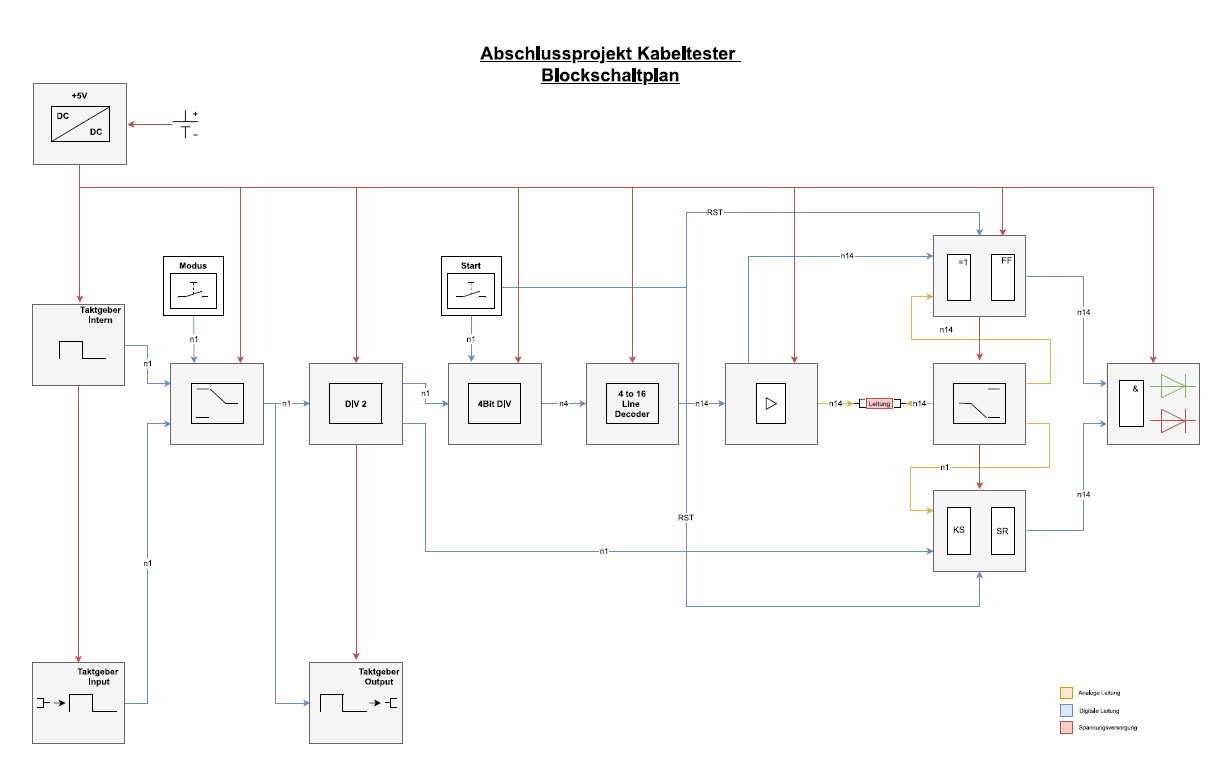
\includegraphics[width=22cm, angle=-90]{Bilder/Blockschaltplan.png}
\end{center}

\newpage

\begin{center}
Die Kernfunktion der Messplatine wird in diesem Dokumentationsteil anhand des Blockschaltbildes erklärt. 
\end{center}

Die Versorgung dieser Platine soll durch einen 9V Batterieblock erfolgen. Die Spannung wird dabei durch einen DC/DC - Wandler auf 5V gewandelt.
\\
\\
Ein interner sowie externen Takt kann Wahlweise als Systemtakt verwendet werden. Über einen Taster kann zwischen diesen Taktquellen umgeschaltet werden.
\\
\\
Um den Systemtakt auf mehreren hintereinander geschalteten Messplatinen verwenden zu können, wird dieser auf einem Stecker herausgeführt.
\\
\\
Der Systemtakt wird nun durch den Faktor zwei geteilt und bildet den Messtakt. Mit diesem Takt werden die einzelnen Adern des zu messenden Kabels geprüft.
\\
\\
Um jede einzelne Ader nach einander messen zu können, wird mit Hilfe des Messtaktes, durch einen 4 Bit Zählerbaustein von 0 bis 15 hochgezählt. Über einen Taster druck kann dieser Zählvorgang gestartet werden und die Ausgänge wieder in einen definierten Zustand gebracht werden.
\\
\\
Der 4Bit Decoder schaltet dabei für jeden möglichen Zählerstand den passenden Ausgang auf High. Läuft keine Messung, so weißen alle Ausgänge ein Low-Pegel auf. 
\\
\\
Da bei der Konstantstrommessung ein Strom bis zu 100mA durch das Kabel fließen kann, steuert der 4 Bit Decoder mit seinen Ausgängen parallele Leistungsstufen an.
\\
\\
Zwischen den Leistungsstufen und dem Analogschalter wird das zu Messende Kabel  (Ader) gesteckt. 
\\
\\
Der Analogschalter ist dafür verantwortlich zwischen der Konstantstrommessung und der Kurzschlussmessung sowie Durchgangsmessung, während der Messung umzuschalten. 
\\
\\
Während der Pausenzeit des Messtaktes, wird ein konstanter Strom durch das Kabel fließen. Mit Hilfe des Spannungsfall über den strombegrenzenden MOSFET der Konstantstromquelle, kann indirekt der Kabelwiderstand bestimmt werden. Das Ergebnis dieser seriellen Messung wird durch ein Schieberegister parallel ausgegeben. Da die Konstantstromquelle bei jedem Kabel den Strom neu regeln muss, wird durch den zugeführten Systemtakt erst nach der Hälfte der Messzeit das Ergebnis via Schiebetakt übernommen.
\\
\\
Während der Impulszeit des Messtaktes, wird das Kabel auf Kurschluss sowie Durchgängigkeit überprüft. 
\\
\\
Liefern beider Messungen einer Ader ein High-Signal, leuchtet eine grüne LED. Liefert eine oder beide Messungen ein Low-Signal, leuchtet die rote LED.




\end{document}
\newpage
\documentclass[a4paper,11pt]{scrartcl}

\usepackage[utf8]{inputenc}
\usepackage[ngerman]{babel}
\usepackage[T1]{fontenc}
\usepackage{amsmath}
\usepackage{graphicx}
\usepackage{tabularx}
\usepackage[a4paper, left=2cm, right=2cm, top=2.8cm, bottom=2.8cm]{geometry}
\usepackage{tikz}   
\usepackage[scaled]{helvet}
\usepackage{tabto} 
\usepackage{fancyhdr}
\usepackage{multirow}

\renewcommand*{\familydefault}{\sfdefault}

\pagestyle{fancy}

\setkomafont{section}{\huge}
\setkomafont{subsection}{\Large}


\lhead{Maximilian Hoffmann}
\chead{Betrieblicher Auftrag \\ \textbf{Kabeltester}}
\rhead{
\includegraphics[width=3cm]{Bilder/BMK_LOGO.png}}

%%%%%%%%%%%%%%%%%%%%%%%%%%%%%%%%%%%%%%%%%%%%%%%%%%%%%%%%%%%%%%%%%%%%%%%%%%%%%%%%%%%%%%%%%%%%%%%%%%%%%%%%%%%%%%%%%%%%%%%%%%%%%%%%%%%%%%%%%%%%%%%																																			 %
%														Funktionen der Schaltung															%
%																																		     %
%%%%%%%%%%%%%%%%%%%%%%%%%%%%%%%%%%%%%%%%%%%%%%%%%%%%%%%%%%%%%%%%%%%%%%%%%%%%%%%%%%%%%%%%%%%%%%%%%%%%%%%%%%%%%%%%%%%%%%%%%%%%%%%%%%%%%%%%%%%%%%

\begin{document}

%%%%%%%%%%%%%%%%%%%%%%%%%%%%%%%%%%%%%%%%%%%%%%%%%%%%%%%%%%%%%%%%%%%%%%%%%%%%%%%%%%%%%%%%%%%%%%%%%%%%%%%%%%%%%%%%%%%%%%%%%																																						%
%														Versorgung														%
%																														%
%%%%%%%%%%%%%%%%%%%%%%%%%%%%%%%%%%%%%%%%%%%%%%%%%%%%%%%%%%%%%%%%%%%%%%%%%%%%%%%%%%%%%%%%%%%%%%%%%%%%%%%%%%%%%%%%%%%%%%%%%

\section{Schaltplanentwurf}

\subsection{Versorgung}

\subsubsection{Schutzbeschaltung}

\begin{center}
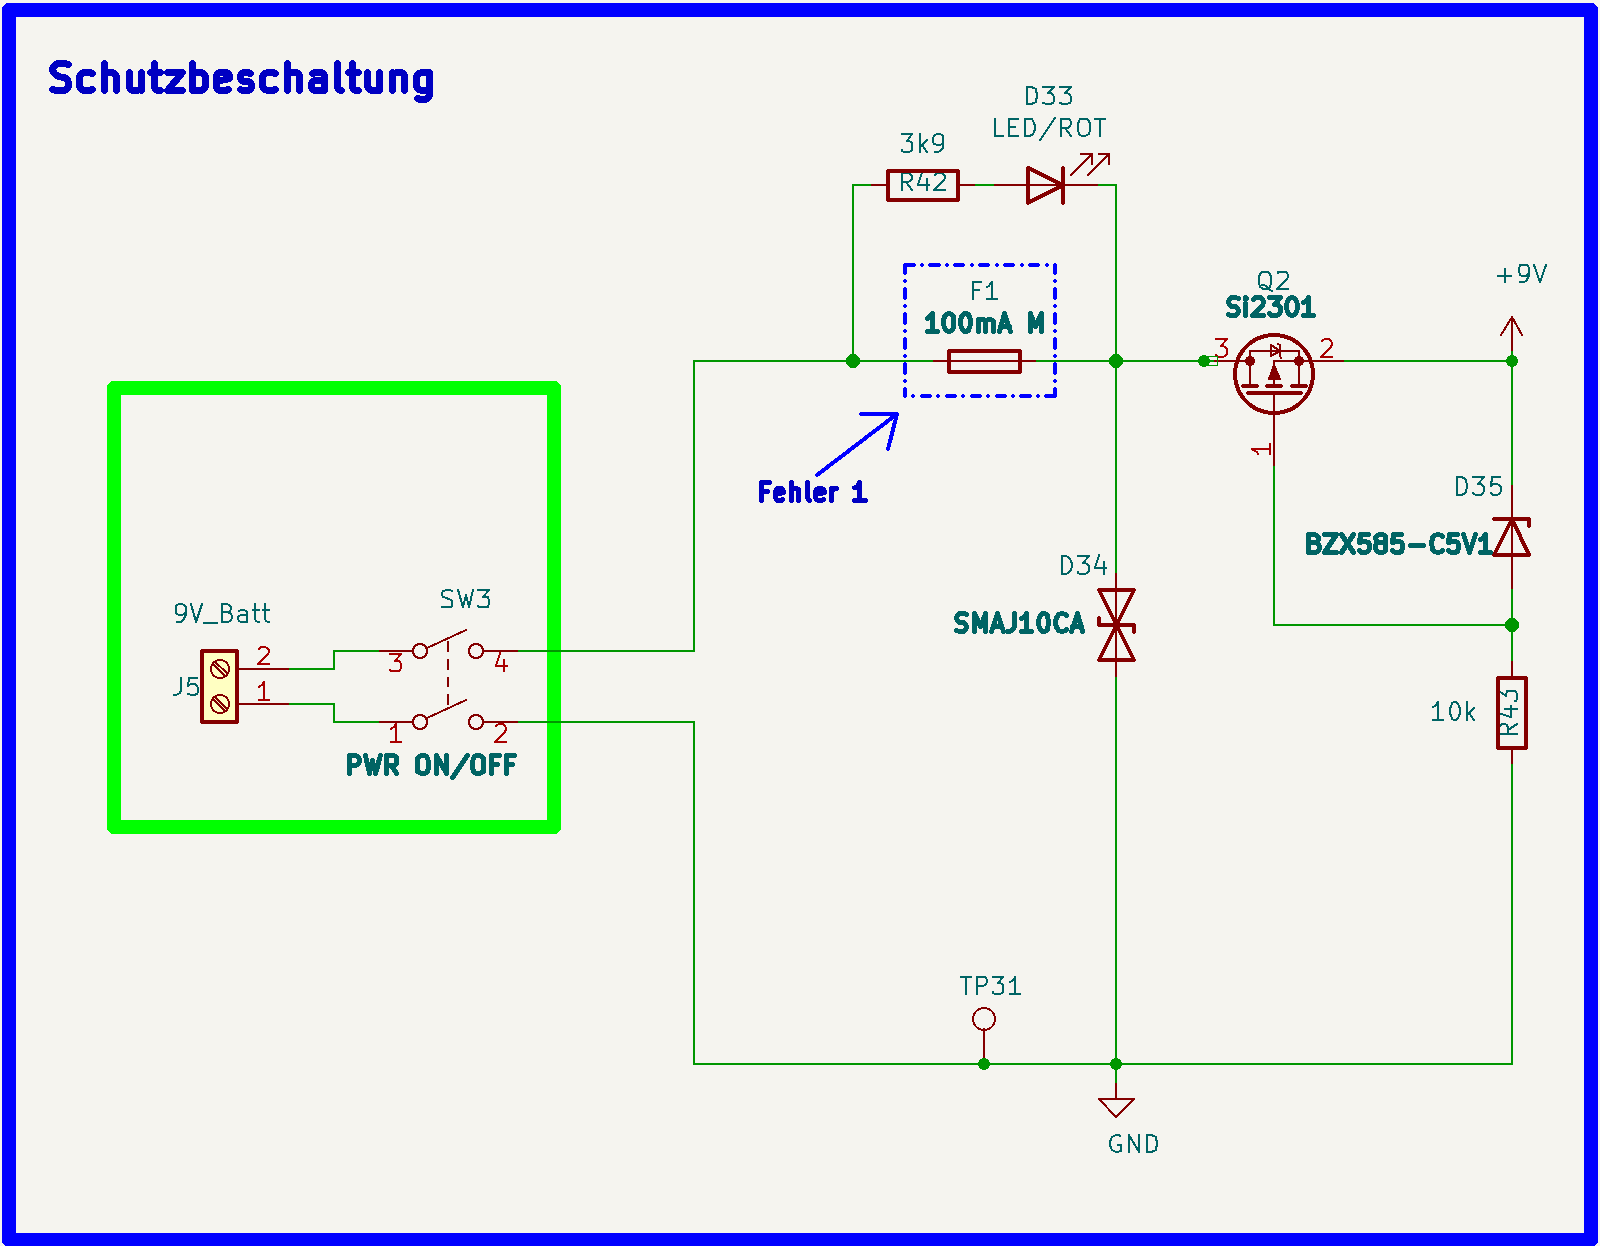
\includegraphics[width=10cm]{Bilder/Schutzbeschaltung.png}
\end{center}

Um die Schaltung zu schützen, wurde auf eine umfangreiche Eingangsschutzbeschaltung gesetzt. Die Versorgungsspannung kann dabei zweipolig durch den Schalter \glqq Power ON/OFF SW3 \grqq{} abgeschaltet werden.
\\
\\
Die mittelträge Sicherung F1, ist für den Überstromschutz verantwortlich. Löst diese aus, so fließt ein Strom über R42 und D33. Dabei wird der gesamte Stromfluss in der Schaltung auf ein Maximum von 2mA begrenzt. Als Ergebnis leuchtet D33 rot.
\\
Im Normalbetrieb werden R42 und D33 durch den ohmschen Widerstand der Sicherung F1 (12R) überbrückt.
\\
\\
Um den Eingang des DC/DC Wandlers vor Überspannungsspitzen zu schützen, kommt eine 10V TVS Diode zum Einsatz. Die Eingangsspannung dieser Schaltung wird dadurch auf ein Spannungsmaximum von 10V begrenzt. 
\\
\\
Da es bei einer Batterieanwendung sehr schnell zu einer ungewollten Verpolung der Anschlüsse kommen kann, wird ein Verpolungsschutz benötigt.
\\
Liegt eine korrekt gepolte Spannung an, so fließt der Strom durch die Z-Diode D35 und den strombegrenzenden Widerstand R43. Die über die Z-Diode abfallende Spannung von 5,1V, liegt somit auch an den Anschlüssen \glqq Source und Gate \grqq{} des P-Channel MOSFET Q2 an.
In diesem Fall, liegt eine um ca. 5V negativere Spannung an Gate gegenüber Source an. Die Drain-Source Strecke leitet und es kann Strom fließen.
\\ 
Wird die Versorgungsspannung verpolt, so fließt der Strom durch den Widerstand R43 und durch die Diode D35. Die Diode D35 befindet sich dabei in Durchlassrichtung und besitzt somit die Eigenschaften einer Si-Diode.
Die Spannung an Gate ist dabei um ca. 5V positiver gegenüber Source. Der P-Channel MOSFET sperrt und unterbindet einen Stromfluss.
\\

\subsubsection{DC/DC Wandler}

\begin{center}
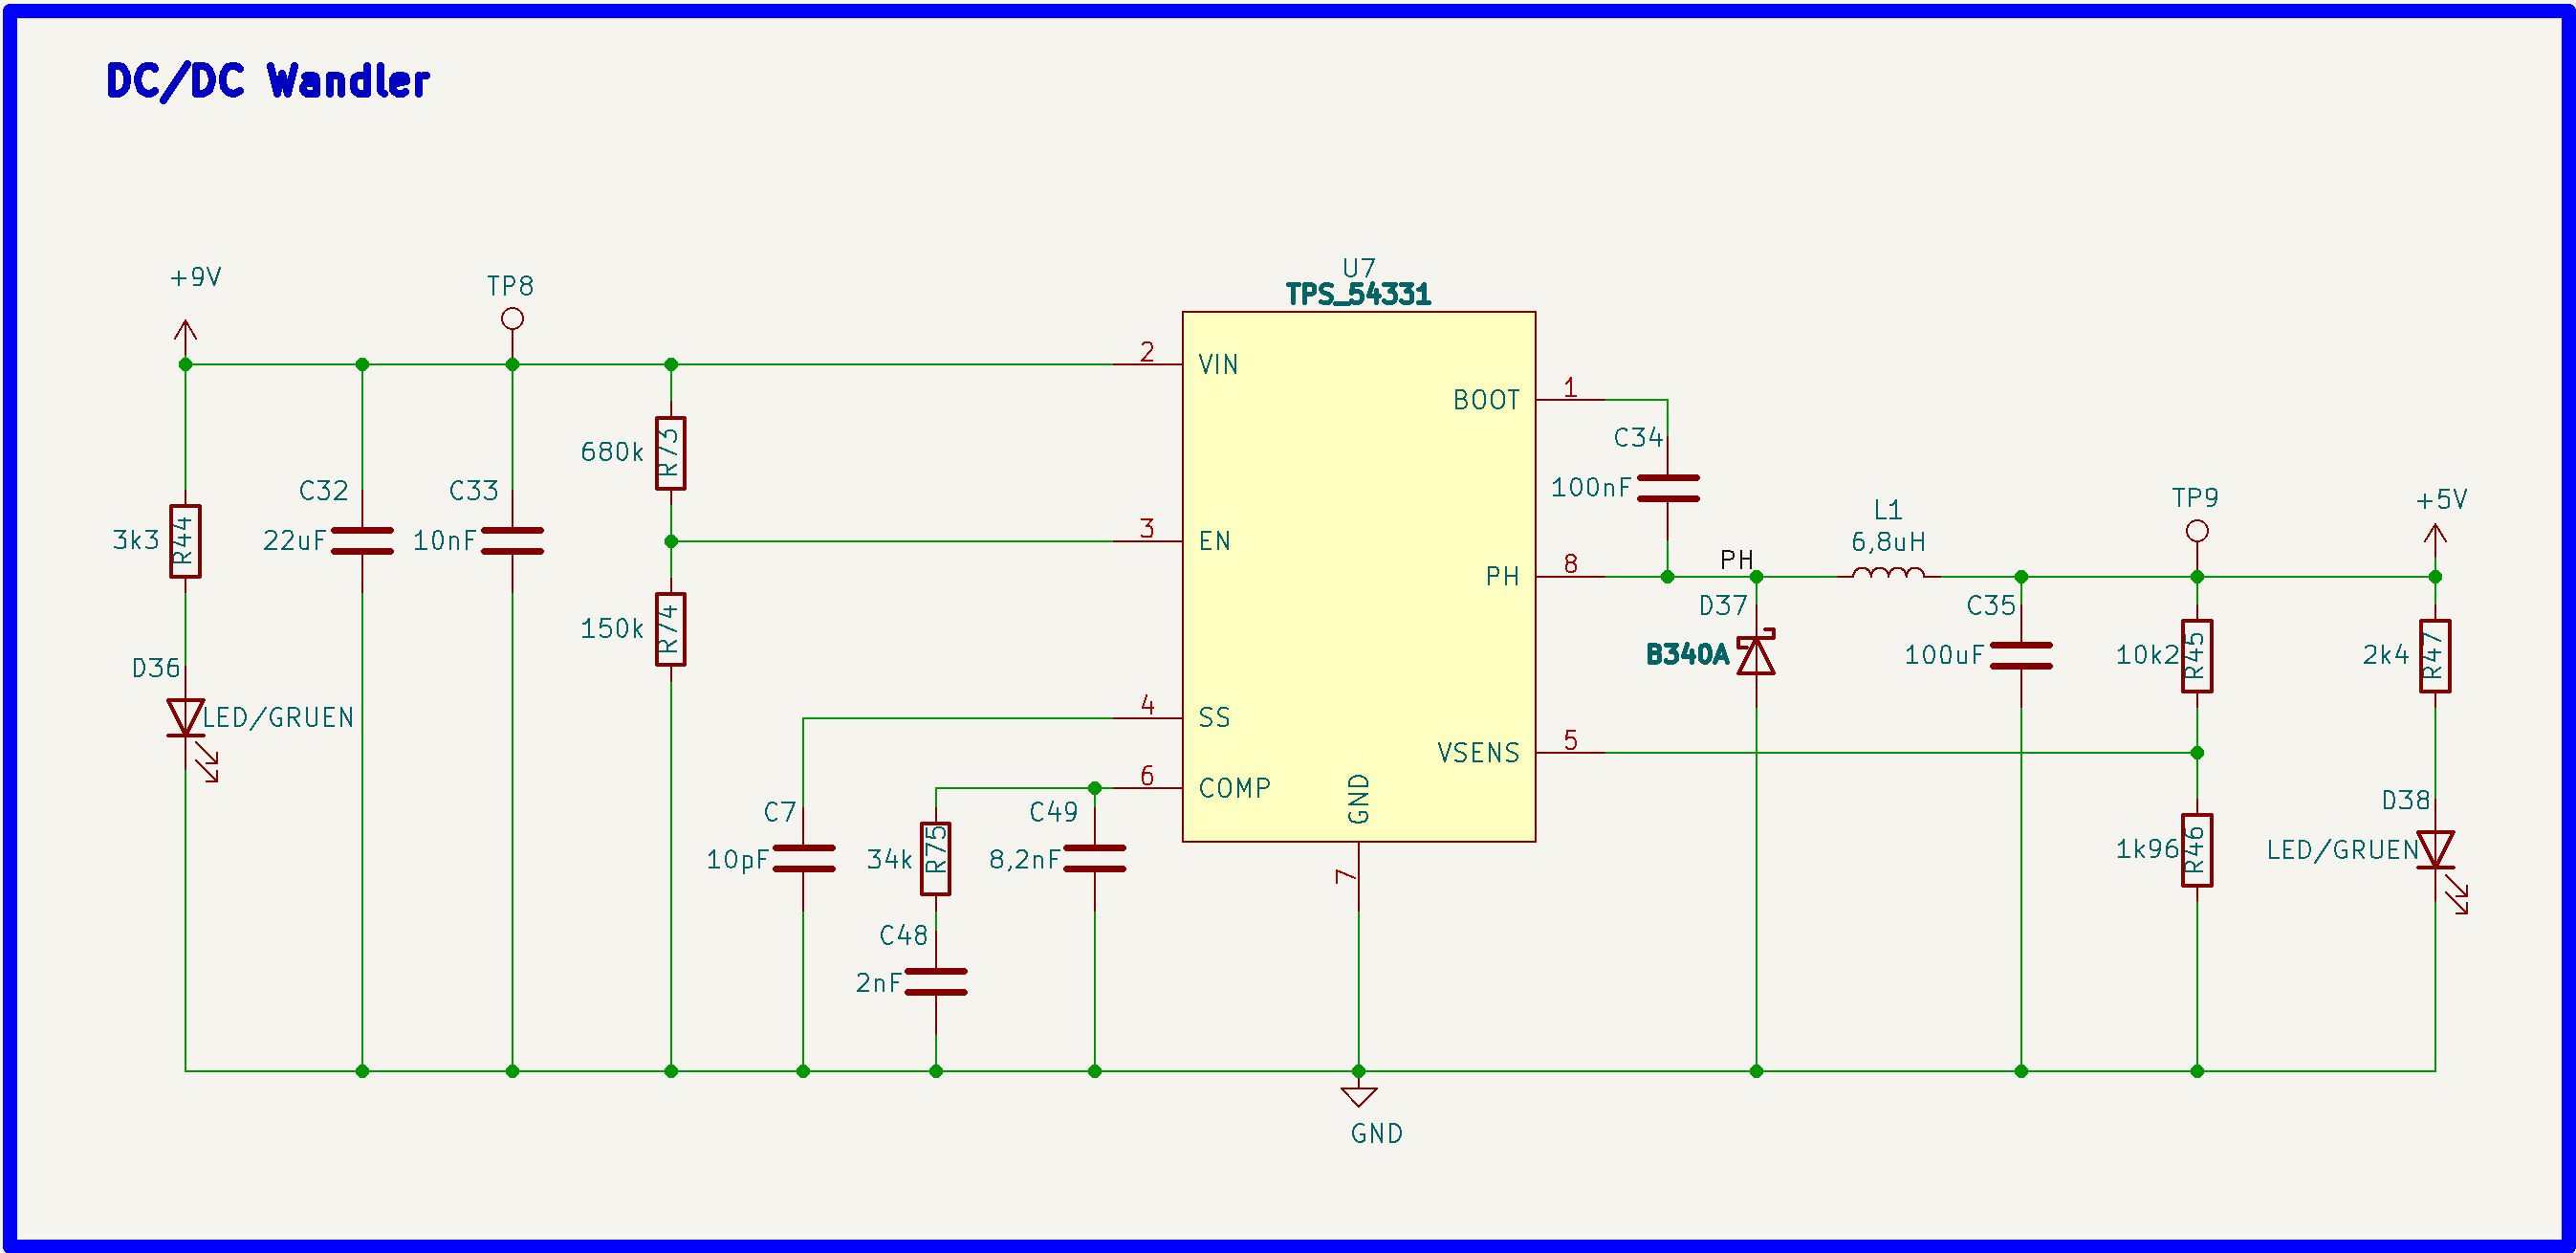
\includegraphics[width=16cm]{Bilder/DCDCWandler.png}
\end{center}

Bei der Auswahl des DC/DC Wandlers wurde auf die Verfügbarkeit bei BMK im Haus geachtet.
\\
Die Dimensionierung der externen Bauelemente wurde mit Hilfe des \glqq Texas Instruments Power Designer\grqq{} Web-Tool durchgeführt.
\\
Die grünen LED's D36 und D38 sorgen für ein optisches Feedback der Versorgungsspannungen.
\\
Allgemein wurde der Wandler für eine Ausgangsspannung von +5V und einen Ausgangsstrom von ca. 1,5A dimensioniert. Mit den Widerständen R73 und R74 kann der Schaltregler bei Über/-Unterspannung abschalten. Dafür wird eine oberer sowie untere Schaltschwelle berechnet.

\begin{center}
\begin{align}
	R73 &= \dfrac{V_{\Delta}}{3uA} = \dfrac{2V}{3uA} = 666k  \Rightarrow 680k\\
	R74 &= \dfrac{1,25V}{\dfrac{Vs - 1,25V}{R73} + 1uA} = \dfrac{1,25V}{\dfrac{8V - 1,25V}{680k} + 1uA} = 126k \Rightarrow 150k	\\
	V_{OUT}	&= V_{REF} + (\dfrac{R45}{R46} + 1) = 0,8V + (\dfrac{10,2k}{1,96k} + 1) = 4,96V
\end{align}
\end{center}


\newpage

%%%%%%%%%%%%%%%%%%%%%%%%%%%%%%%%%%%%%%%%%%%%%%%%%%%%%%%%%%%%%%%%%%%%%%%%%%%%%%%%%%%%%%%%%%%%%%%%%%%%%%%%%%%%%%%%%%%%%%%%%																																						%
%														NE555 Taktgeber													%
%																														%
%%%%%%%%%%%%%%%%%%%%%%%%%%%%%%%%%%%%%%%%%%%%%%%%%%%%%%%%%%%%%%%%%%%%%%%%%%%%%%%%%%%%%%%%%%%%%%%%%%%%%%%%%%%%%%%%%%%%%%%%%

\subsection{NE555 Taktgeber}

\subsubsection{Takt}

\begin{center}
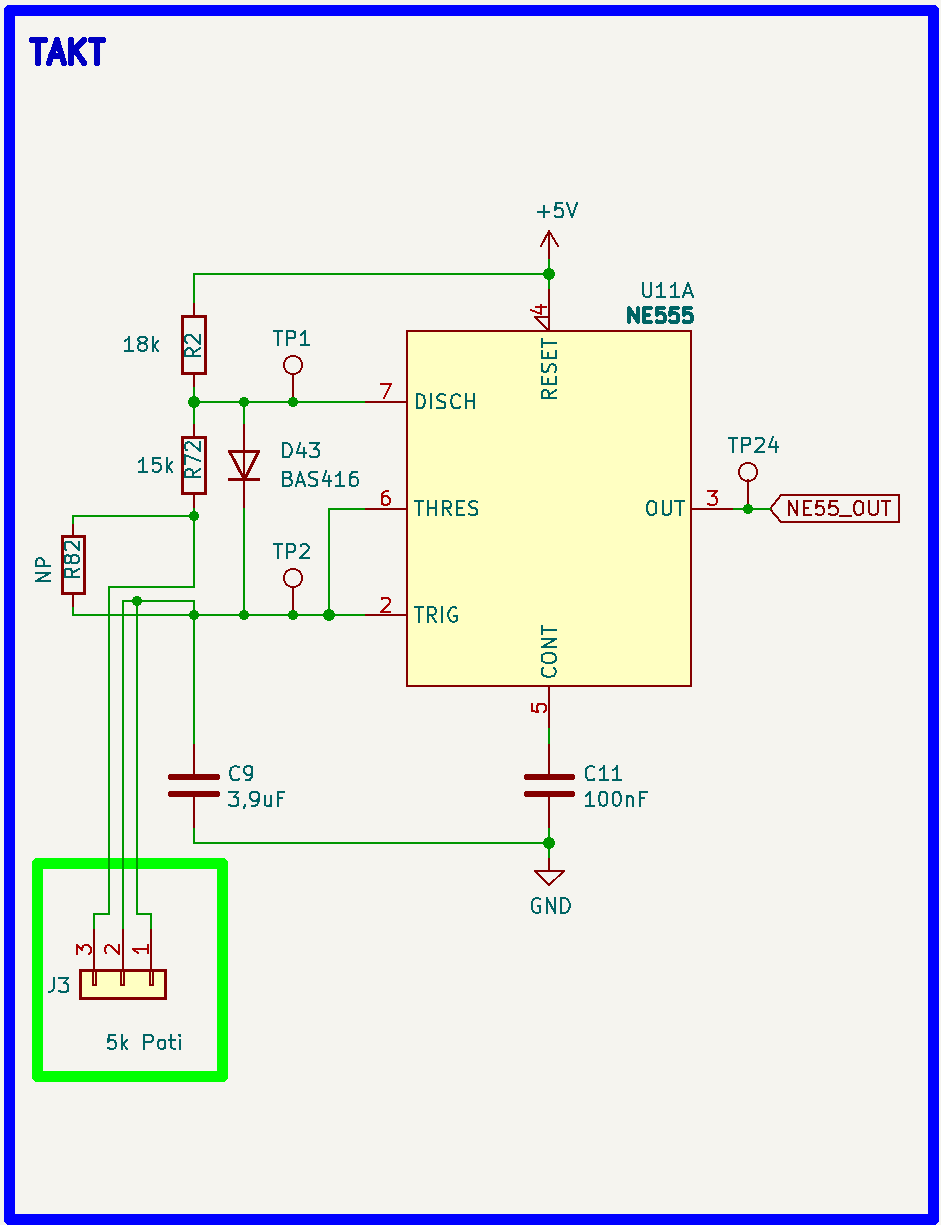
\includegraphics[width=10cm]{Bilder/Takt.png}
\end{center}

Als Taktgeber kommt der \glqq NE555 \grqq{} zum Einsatz. Dieser wird als astabile Kippstufe betrieben. Mit Hilfe der Diode D43 gleichen sich Impulszeit und Pausenzeit an. Über das Poti (Connector) J3 soll die Ausgangsfrequenz auf ca. 10Hz eingestellt werden können. 
\\
\\
Im Einschaltmoment ist C9 entladen. Somit liegt das Signal am Triggereingang (PIN 2) unterhalb von $\frac{1}{3} VCC$. Das interne FlipFlop wird gesetzt und der Ausgang (PIN 3) erfährt einen High-Pegel. Der Kondensator C9 lädt sich nun über den Strompfad R2 und D43 auf. Der Ladevorgang hält so lange an, bis das Spannungspotential an Pin 6 (Threshold) einen höheren Wert als $\frac{2}{3} VCC$ aufweist. Das interne FlipFlop's wird zurückgesetzt und der Ausgang erfährt einen Low-Pegel. Der Kondensator C9 entlädt sich nun über R72 und den (auf GND durchgeschaltenen) Pin 7 (Discharge). Hat sich der Kondensator nun wieder auf ein Spannungspotential unterhalb von $\frac{1}{3}$ entladen, so wird er Ausgang wieder gesetzt und der Entladevorgang über Pin 7 unterbunden. Dieser Vorgang wiederholt sich solange Energie von außen hinzugefügt wird. 

\begin{center}
\begin{align}
	f_{OUT} &= \dfrac{1}{0,69*R2*C9 + 0,69*(R72+R_{J3})* C9} = \dfrac{1}{0,69*18k*3,9uF*2} = 10,3Hz
\end{align} 
\end{center}

\newpage
\subsubsection{Taktumschaltung}

\begin{center}
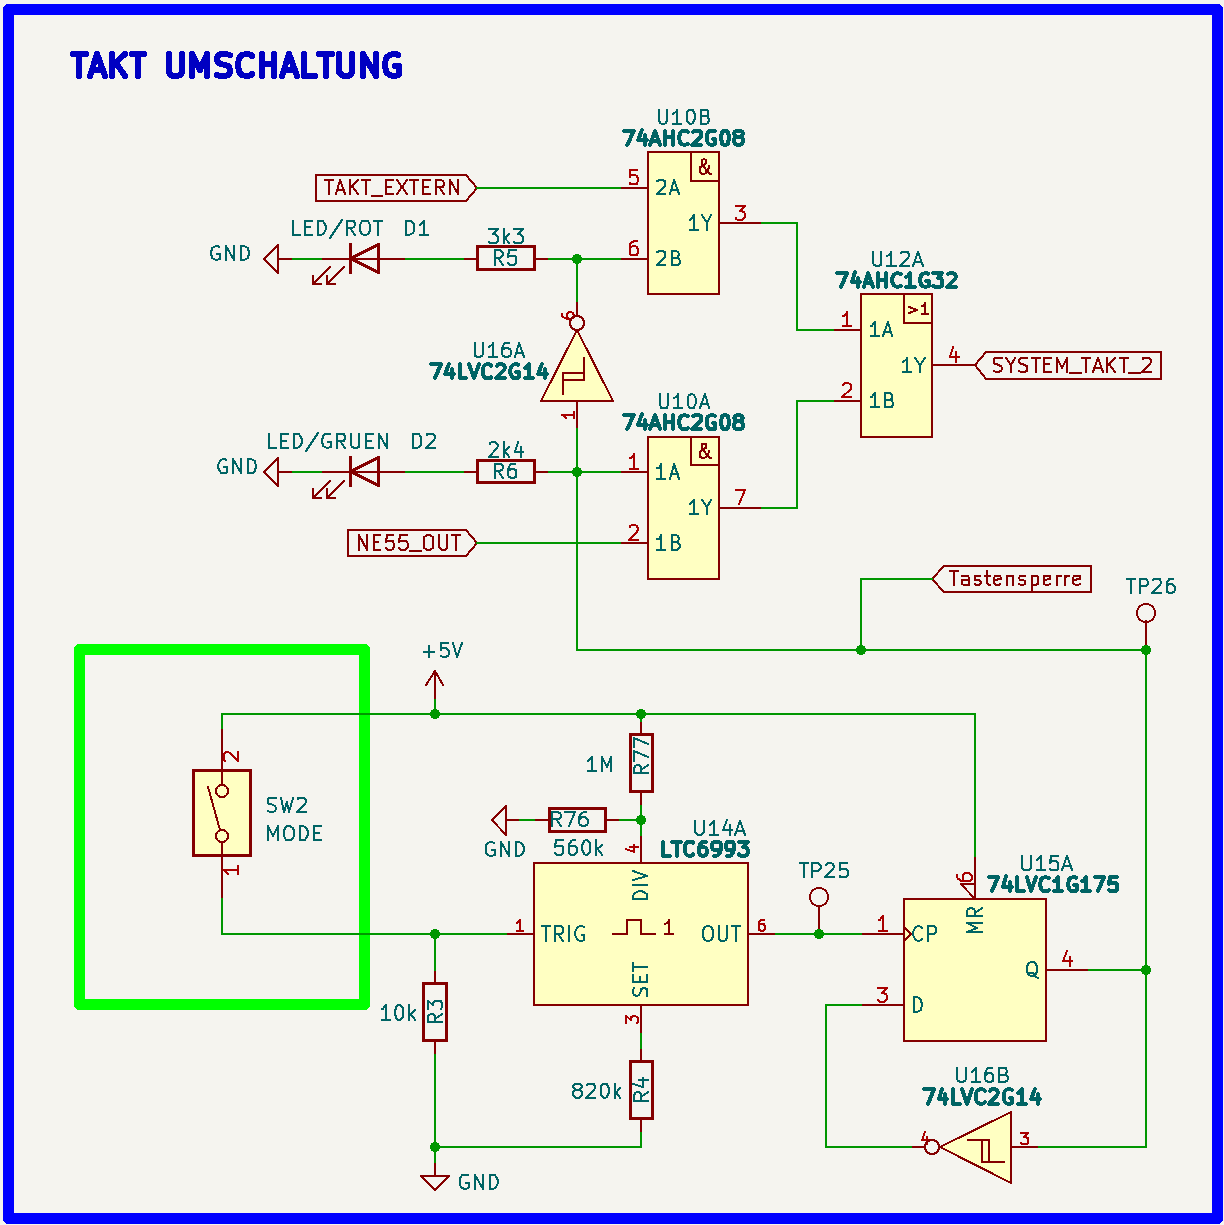
\includegraphics[width=13cm]{Bilder/Taktumschaltung.png}
\end{center}


\textbf{Funktionsbeschreibung LTC6993 U14}
\\
Das IC „LTC6993“ ist eine Monostabile Kippstufe mit einer einstellbaren Pulsweite von 1us – 33,6s. Dabei wird bei einem Impuls über den Trigger-Eingang (Pin 1), der Ausgangszustand für eine einstellbare Zeit gespeichert bevor der Ausgang wieder in den stabilen Zustand zurück kippt. Über die Außenbeschaltung der Pin’s „DIV“ und „SET“ kann die Pulsweite (Kipp-Zeit) konfiguriert werden. Der Pin „DIV“ ist dabei intern mit einem 4 Bit A/D-Wandler beschalten. Dieser führt drei seiner Datenleitungen einem Taktteiler zu. Dieser Taktteiler ist dadurch zwischen 1 und 2 097 152 einstellbar. Die vierte Datenleitung (MSB) übergibt ihren Zustand dem Block „Output Polarity“. Dieser bestimmt den stabilen Ausgangspegel des Monoflops. Ein Widerstand zwischen GND und dem Pin „SET“ ist dabei für die Oszillator-Frequenz zuständig. Die Spannung zwischen „SET“ und GND wird dabei konstant auf 1V gehalten, was einen konstanten Stromfluss hervorruft. Die dabei möglichen Widerstandswerte liegen zwischen 50k und 800k (1,25uA-20uA), was einem Frequenzbereich von 1Mhz bis 62,5kHz entspricht. Die durch den Taktteiler geteilte Oszillatorfrequenz, setzt dabei ein RS-FlipFlop periodisch zurück. Ein Impuls am Trigger-Eingang setzt das FlipFlop, so dass es erst nach einer bestimmten Kipp-Zeit zurückgesetzt werden kann. Der FlipFlop-Ausgang ist dabei über den „Output Polarity“ Block mit dem Ausgang des IC‘s verbunden.

\newpage

\textbf{Funktion}
\\
Der Schaltungsteil \glqq Taktumschaltung \grqq{} ist für das Umschalten der zwei Taktquellen verantwortlich. Es kann zwischen den intern (durch den NE555 generierten) Takt und externen (durch eine vorgeschaltene Messplatine zugeführten) Takt umgeschalten werden . Ausschlaggebend dafür sind zwei Schaltungsteile. Durch betätigen des Tasters SW2 (MODE), wird zwischen den Taktquellen umgeschaltet. Da jede Tasterbetätigung ein mechanisch verursachtes prellen der Kontakte verursacht, muss dies durch das nachgeschaltete  Monoflop (U14) unterbunden werden. Die Zeit, die das Monoflop benötigt mit seinem Ausgang auf einen eingangsseitigen Triggerimpuls zu reagieren, dauert länger als das prellende Signal selbst. Somit kann am Ausgang des Monoflops eine saubere Signalflanke zustande kommen. 
\\
\\
Das nachgeschaltete D-FlipFlop ist in seiner Verschaltung, mit den auf den Dateneingang zurückgeführten invertierten Ausgang, als Toggle FlipFlop zu betrachten. Für einen Pegelwechsel am Ausgang Q des Toggle FlipFlop ist eine steigende und fallende Flanke notwendig. Eine Betätigung mit zwei dynamischen Flanken verursacht demnach einen Pegelwechsel an TP28 mit nur einer dynamischen Flanke. 
\\
\\
Die auf TP28 folgende Schaltung ist als zweifach TOR-Schaltung mit nur einem Steuereingang zu verstehen. Ein High-Signal an TP28 führt dazu, dass die an den Pin 2 (U10A) anliegenden Taktsignale auf den Ausgang übertragen werden. Durch die Invertierung von TP28 werden Taktsignale, die an Pin 5 (U10B) anliegen unterdrückt. Der Ausgang bleibt Low.
\\
Ein Low-Signal an TP28 führt zur unterdrückung der an Pin2 (U10A) anliegenden Signale. Das durch eine vorgeschaltene Messplatine der Schaltung ugeführte Signal an Pin 5 (U10B) wird nun an den Ausgang übertragen.
\\
Das Oder-Gatter überträgt entweder das Signal von U10B oder das Signal von U10A auf seinen Ausgang. 

\newpage

\subsubsection{Taktteilung}

\begin{center}
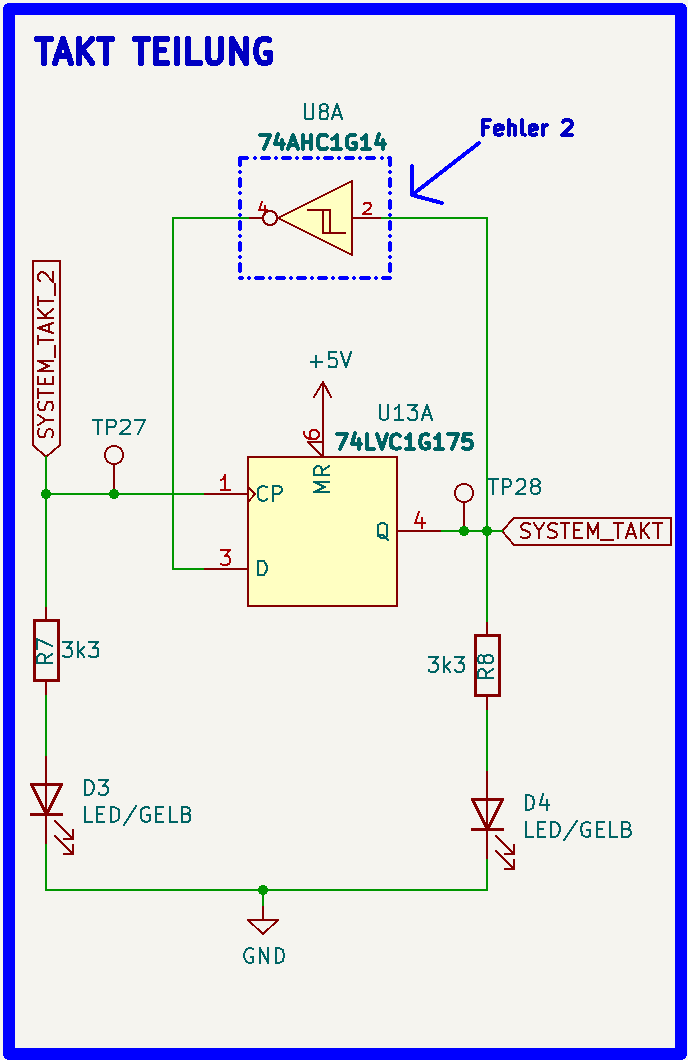
\includegraphics[width=7cm]{Bilder/Taktteilung.png}
\end{center}

Für einen folgenden Schaltungsteil wird ein Takt, welcher die doppelte Frequenz des Messtaktes besitzt benötigt. Dazu wird der Grundtakt durch zwei geteilt und als Messtakt verwendet. Der externe oder interne Grundtakt wird vom folgenden Schaltungsteil verwendet.
\\
D3 und D4 geben ein optisches Feedback des Mess- und Grundtaktes. 


\subsection{Dezimal Zähler}

\subsubsection{Messung Starten}

\begin{center}
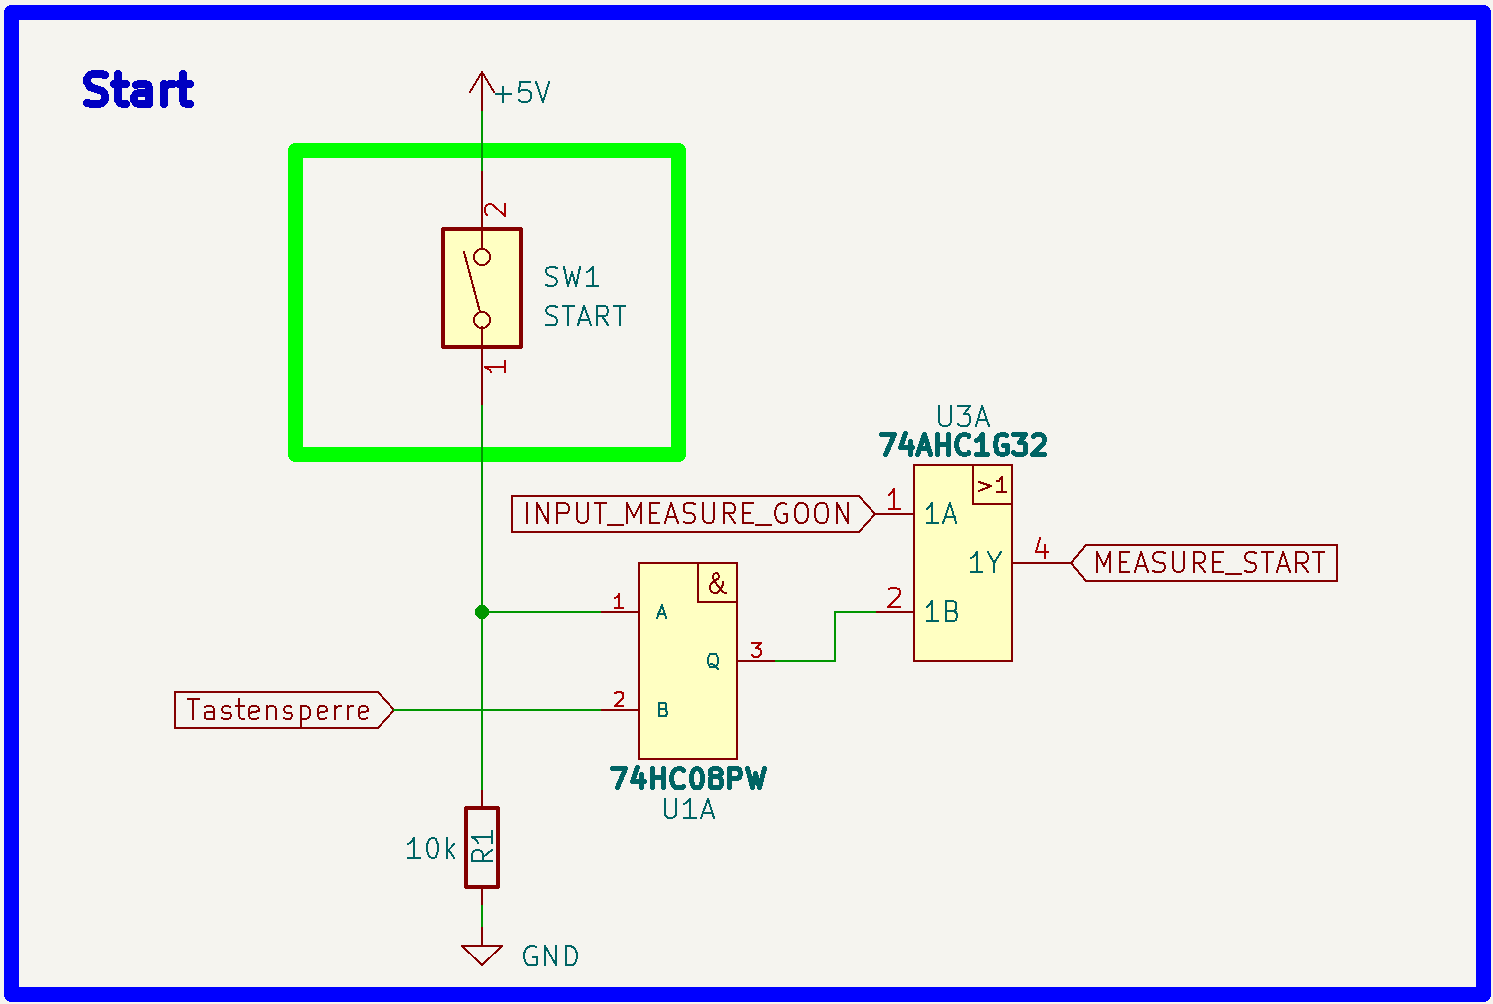
\includegraphics[width=12cm]{Bilder/Start.png}
\end{center}

Die Messung kann über Betätigung des Tasters SW1 (START) oder über ein externes Signal (Label: INPUT MEASURE GOON) gestartet werden. Befindet sich die Messplatine im \glqq Master Mode \grqq{} (\textbf{Master Mode:}  Grundtakt = Interner Takt \textbf{Slave Mode:} Grundtakt = Externer Takt), so kann die Messung durch den Tasters SW1 gestartet werden. Befindet sich die Messplatine im \glqq Slave Mode \grqq{} so kann nur durch ein externes Signal die Messung gestartet werden. Der Taster SW1 (START) ist gesperrt.


\subsubsection{Reset}

\begin{center}
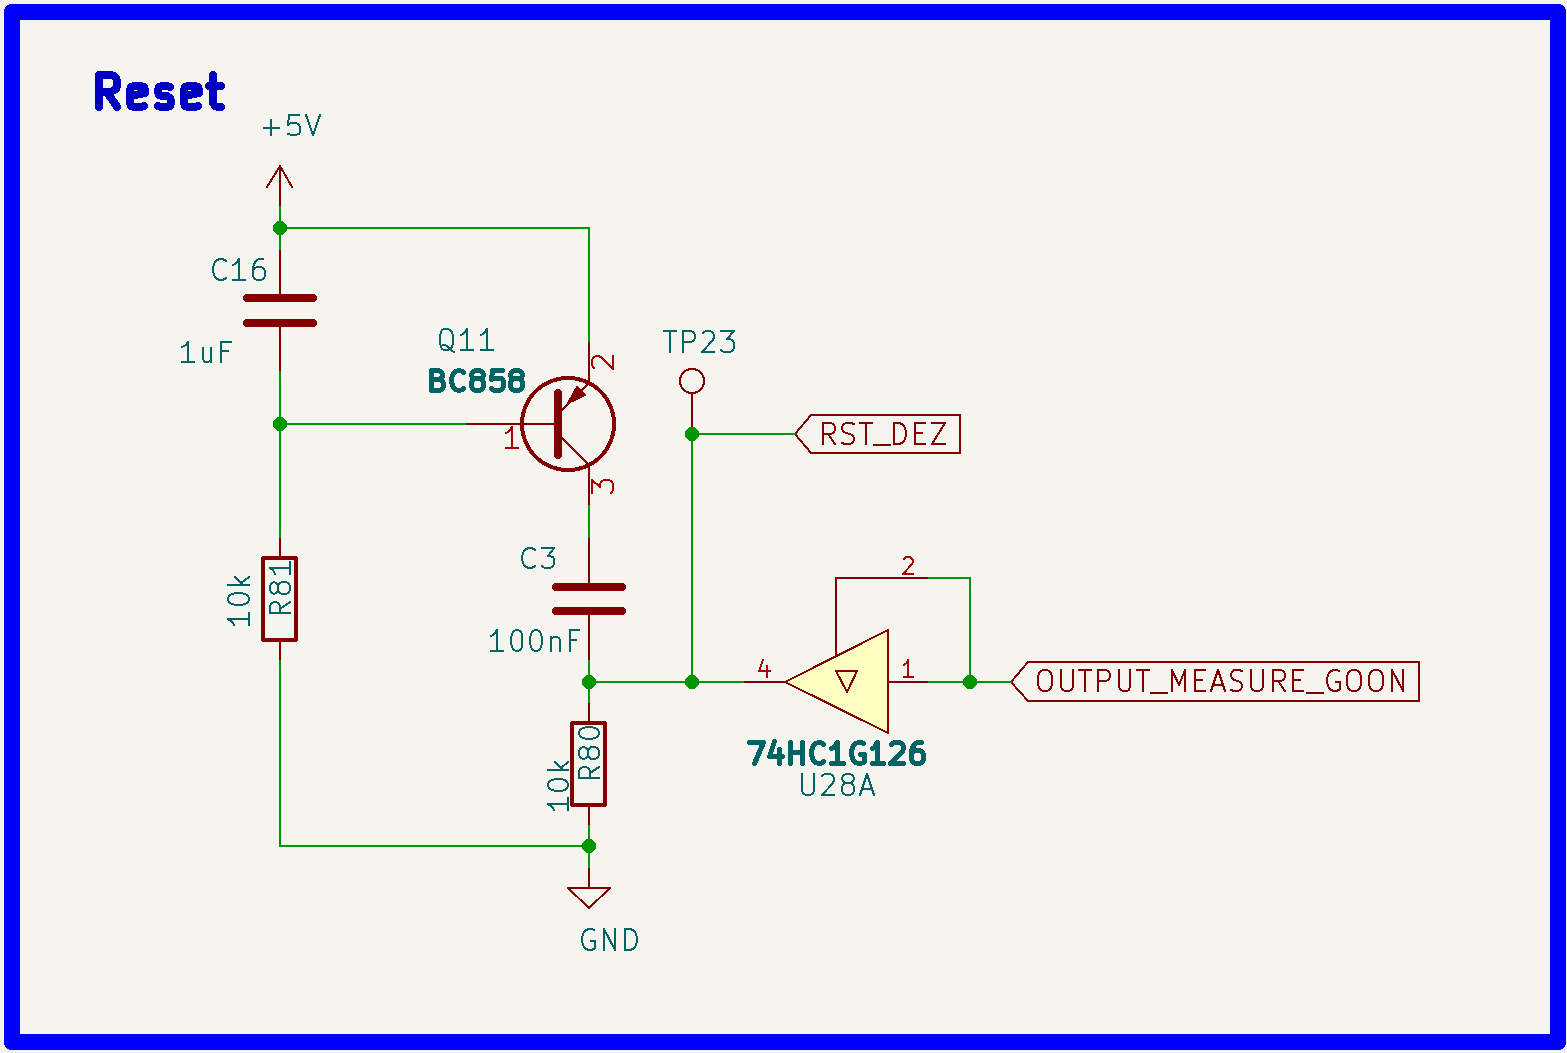
\includegraphics[width=12cm]{Bilder/Reset.png}
\end{center}

Die Aufgabe der folgenden Schaltung besteht darin, kurze Zeit nach dem Einschalten einen Reset-Impuls für ausgewählte Schaltungsteile zu generieren. Wird dies nicht gemacht, so kann es unter zufälligen Umständen sein, dass die Messung nicht gestartet werden kann.
\\
\\
Im Einschaltmoment fließt Strom über C16 und R81. C16 liegt dabei parallel zu den Anschlüssen \glqq Emitter und Basis\grqq{} des PNP-Transistors Q11. Da im Einschaltmoment C16 als Kurzschluss zu betrachten ist, liegen Emitter und Basis auf dem selben Potential. Ein Stromfluss ist daher nicht möglich und der Transistor Q11 sperrt. C16 beginnt sich über die Zeit langsam aufzuladen. Liegt ein bestimmtes Spannungspotetial über C16 an (ca. 0,7V $U_{BE}$), so ist ein Stromfluss durch die Basis möglich. Nach einer bestimmten Verzögerung ist nun auch ein Stromfluss durch den Transistor Q11, dem Kondensator C5 und dem Widerstand R80) möglich. Da C3 ebenfalls im ersten Moment als Kurzschluss zu betrachten ist, fällt über R80 angfänglich ein 5V pegel ab. Die Spannung über C3 baut sich dabei sehr schnell auf, was einen kurzen Nadelimpuls zur folge hat. Das globale Label \glqq RST DEZ\grqq{} resetet die Schaltungsteile.  
\\
\\
Das IC U28A dient zur Stromkreisentkopplung und soll beim Resetvorgang einen Kurzschluss vermeiden.

\newpage
\subsubsection{Controlling}

\begin{center}
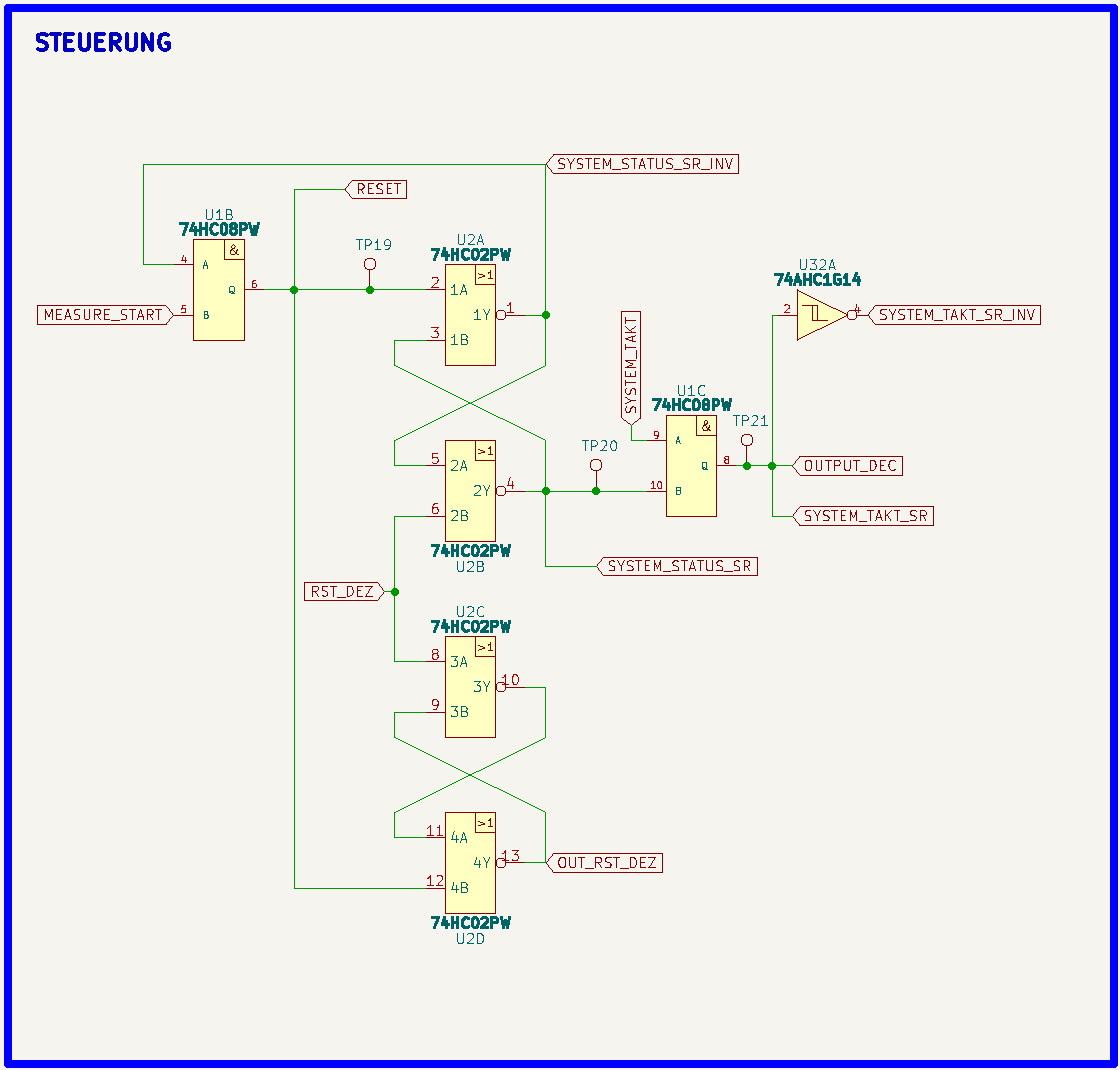
\includegraphics[width=12cm]{Bilder/Controlling.png}
\end{center}

Durch die voran gegangene Schaltung, welche die FlipFlops \textbf{FF1:} U2A und U2B \textbf{FF2:} U2C und U2D in die definierten Ausgangszustände bringt, kann nun ein einwandfreier Start der Messung durchgeführt werden. 
\\
\\
Zum Start der Messung hat das IC U2A einen Ausgangsseitigen High-Pegel vorzuweisen. Der Ausgang ist dabei auf den Steuereingang des TOR-Gatter zurückgeführt.
\\
Das TOR-Gatter U1C erfährt an seinem Steuereingang Pin 10 einen Low-Pegel. Der anliegende Messtakt wird gesperrt.
\\
An dem Ausgang des IC U2D liegt ein Low-Signal an. Dieses Low-Signal resetet die folgende Schaltung dauerhaft.  
\\
\\
Ein High-Signal am Pin 5 (U1B \textbf{LABEL:} MEASURE START) wird auf den Ausgang übertragen. Das an TP19 zu messende High-Signal bleibt so lange aktiv, wie das folgende FlipFlop (U2A und U2B) für das Rücksetzen des Ausganges Pin 1 bzw. für das Setzen des Ausganges Pin 4 benötigt (Gatterlaufzeit). Ein eventuell prellendes Signal an U1B wird somit sofort unterdrückt.
\\
Das High-Signal an TP20 führt dazu, dass der Messtakt an Pin 8 (U1C) auf den Ausgang übertragen wird. 
\\ 
Der Nadelimpuls an TP19, führt somit zu einem Rücksetzen des IC U2D. Das daraus resultierende Low-Signal gibt die Folgeschaltung somit frei. 


\end{document}
\newpage
\section{Inbetriebnahme}



Die Inbetriebnahme der Schaltung erfolgt blockweise. Um gegebenenfalls Fehler in der Schaltung analysieren zu können, werden die einzelnen Schaltungsteile nacheinander aufgebaut und in Betrieb genommen. Die Funktion der zu prüfenden Schaltungsteile wird oberhalb der Tabelle in Stichpunkten erläutert. Bei fehlerhafter Funktion wird diese in der Sektion \glqq Fehleranalyse\grqq{} behandelt.



%%%%%%%%%%%%%%%%%%%%%%%%%%%%%%%%%%%%%%%%%%%%%%%%%%%%%%%%%%%%%%%%%%%%%%%%%%%%%%%%%%%%%%%%%%%%%%%%%%%%%%%%%%%%%%%%%%%%%%%%%																																				%
%														Spannungsversorgung												%
%																														%
%%%%%%%%%%%%%%%%%%%%%%%%%%%%%%%%%%%%%%%%%%%%%%%%%%%%%%%%%%%%%%%%%%%%%%%%%%%%%%%%%%%%%%%%%%%%%%%%%%%%%%%%%%%%%%%%%%%%%%%%%

\subsection{Spannungsversorgung}

%%%%%%%%%%%%%%%%%%%%%%%%%%%%%%%%%%%%%%%%%%%%%%%%%%%%%%%%%%%%%%%%%%%%%%%%%%%%%%%
%																			  %
%								Vorgaben									  %
%																			  %
%%%%%%%%%%%%%%%%%%%%%%%%%%%%%%%%%%%%%%%%%%%%%%%%%%%%%%%%%%%%%%%%%%%%%%%%%%%%%%%

\begin{itemize}
	\item{Spannungen sowie Ströme sind hierbei mit einem Multimeter zu messen.}
	
	\item{Die Funktion der \glqq Meldeleuchte Sicherung\grqq{}  wird durch das Entnehmen der Sicherung aus dem Sockel geprüft. Leuchtet die LED D33 auf, so ist die Funktion dieses Schaltungsteiles gegeben.}
	
	\item{Die Funktion des Verpolungsschutz wird durch das Anlegen einer verpolten Spannung geprüft. Dabei sollte die Strombegrenzung des Labornetzteiles auf ca. 5mA eingestellt sein. Geht das Netzteil bei diesem Test nicht in die Strombegrenzung, so ist die Funktion dieses Schaltungsteiles gegeben.}
\end{itemize}

%%%%%%%%%%%%%%%%%%%%%%%%%%%%%%%%%%%%%%%%%%%%%%%%%%%%%%%%%%%%%%%%%%%%%%%%%%%%%%%
%																			  %
%								Tabelle  									  %
%																			  %
%%%%%%%%%%%%%%%%%%%%%%%%%%%%%%%%%%%%%%%%%%%%%%%%%%%%%%%%%%%%%%%%%%%%%%%%%%%%%%%

\renewcommand{\arraystretch}{2}
\begin{tabularx}{\textwidth}{p{0.2\textwidth}| p{0.6\textwidth} | p{0.05\textwidth} | p{0.1\textwidth}}

 &  & i.o & n.i.o \\

\hline

Stromaufnahme & $I_{G}$: \textcolor{blue}{2,7mA} 			& [x] & [ ] \\

\hline

\multirow{3}{*}{Spannungen}
		& $U_{0}$:   \textcolor{blue}{9,46V}				&	[x] & [ ] 	\\
		& $U_{TP8}$: \textcolor{blue}{9,43V}				&	[x]	& [ ] 	\\
		& $U_{TP9}$: \textcolor{blue}{4,91V}				&	[x] & [ ]  	\\
		
\hline		
		
\multirow{2}{*}{Funktionen}
		& Meldeleuchte Sicherung:  		& [x] & [ ] 	\\
		& Verpolungsschutz:				& [x] & [ ] 	\\ 

\end{tabularx}
\renewcommand{\arraystretch}{1}

\begin{figure}[htb]
    \centering
    \begin{minipage}[t]{0.45\linewidth}
        \centering
        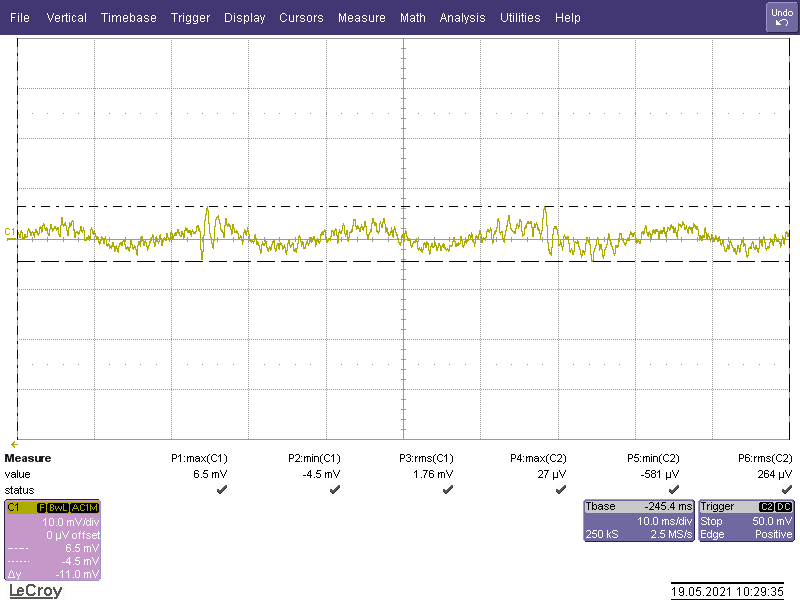
\includegraphics[width=9cm]{Bilder/Versorgungsspannung.png}
        \caption{Versorgungsspannung 5V \\ 11mV Rippelspannung}
    \end{minipage}% <- sonst wird hier ein Leerzeichen eingefügt
   
\end{figure}


%%%%%%%%%%%%%%%%%%%%%%%%%%%%%%%%%%%%%%%%%%%%%%%%%%%%%%%%%%%%%%%%%%%%%%%%%%%%%%%%%%%%%%%%%%%%%%%%%%%%%%%%%%%%%%%%%%%%%%%%%																																				%
%														Taktgeber       												%
%																														%
%%%%%%%%%%%%%%%%%%%%%%%%%%%%%%%%%%%%%%%%%%%%%%%%%%%%%%%%%%%%%%%%%%%%%%%%%%%%%%%%%%%%%%%%%%%%%%%%%%%%%%%%%%%%%%%%%%%%%%%%%

\newpage
\subsection{Taktgeber}

%%%%%%%%%%%%%%%%%%%%%%%%%%%%%%%%%%%%%%%%%%%%%%%%%%%%%%%%%%%%%%%%%%%%%%%%%%%%%%%
%																			  %
%								Vorgaben									  %
%																			  %
%%%%%%%%%%%%%%%%%%%%%%%%%%%%%%%%%%%%%%%%%%%%%%%%%%%%%%%%%%%%%%%%%%%%%%%%%%%%%%%

\begin{itemize}
	\item{Überprüfung der Systemtakte mit Hilfe eines Logikanalysators.}
	
	 \item{Über das Poti soll an TP24 eine Frequenz von 8,5Hz (+-$10\%$) mit einem Tastgrad von 0,5 eingestellt werden.}
	 
	 \item{Durch Betätigen von SW2 kann der Pegel von TP26 gewechselt werden, was durch das optische Signal von D1 oder D2 erkennbar wird.}
	 
	 \item{Die Aufgabe von U14 ist die Signalentprellung des Tasters SW2. Diese Funktion wird durch das oszillieren der Signale U14 Pin 1 und TP25 überprüft. Die Kippzeit des Monoflops soll ca. 500ms betragen.}
	 
	 \item{Leuchtet D2 (Grün), so soll an TP27 die Frequenz von TP24 zu messen sein. Die zu messende Frequenz von TP28 soll dabei die Hälfte von TP27 betragen. Leuchtet D1 (Rot), so soll (sofern kein Verbund aus zwei Messplatinen besteht) keine Frequenz an TP27 und TP28 zu messen sein.}	 
\end{itemize}

%%%%%%%%%%%%%%%%%%%%%%%%%%%%%%%%%%%%%%%%%%%%%%%%%%%%%%%%%%%%%%%%%%%%%%%%%%%%%%%
%																			  %
%								Tabelle  									  %
%																			  %
%%%%%%%%%%%%%%%%%%%%%%%%%%%%%%%%%%%%%%%%%%%%%%%%%%%%%%%%%%%%%%%%%%%%%%%%%%%%%%%

\renewcommand{\arraystretch}{2}
\begin{tabularx}{\textwidth}{p{0.2\textwidth}| p{0.6\textwidth} | p{0.05\textwidth} | p{0.1\textwidth}}

 &  & i.o & n.i.o \\

\hline

Stromaufnahme & $I_{G}$: \textcolor{blue}{6,3mA} & [x] & [ ] \\

\hline

\multirow{2}{*}{Frequenz NE555 }
		& $f_{TP24}$: \textcolor{blue}{8,44Hz}				& [x] & [ ] \\
		& $g_{TP24}$: \textcolor{blue}{0,63}				& [x] & [ ] \\

\hline

\multirow{2}{*}{Taktumschaltung}
		& Taktumschaltung:									&	[x] & [ ] 	\\
		& $t_{Kippzeit}$: \textcolor{blue}{539ms}			&	[x]	& [ ] 	\\
	
\hline		
		
\multirow{3}{*}{Funktionen}
		& Funktion wenn D2 (Grün) leuchtet:  			& [ ] & [x] 	\\
		& $f_{TP28}$: 	\textcolor{blue}{4,23Hz}		& [x] & [ ] 	\\
		& Funktion wenn D1 (ROT) leuchtet:				& [x] & [ ] 	\\ 

\end{tabularx}
\renewcommand{\arraystretch}{1}

\begin{figure}[htb]
    \centering
    \begin{minipage}[t]{0.45\linewidth}
        \centering
        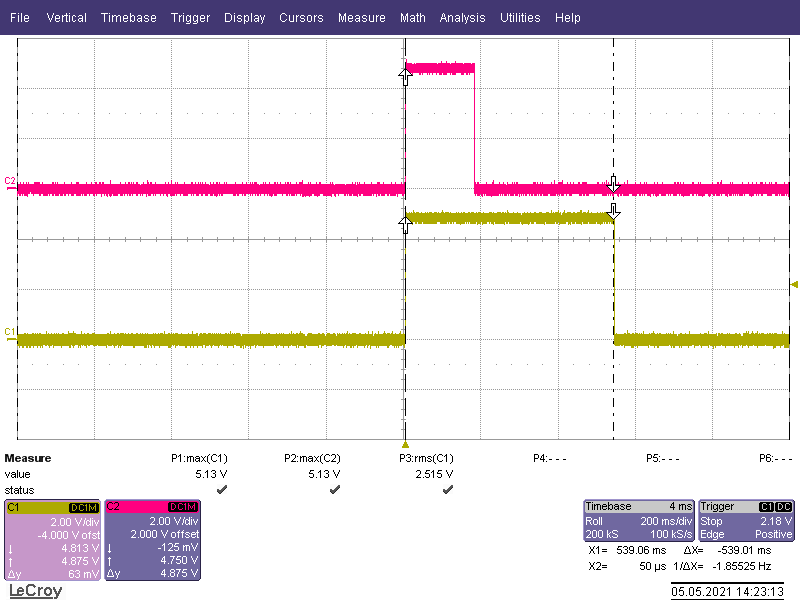
\includegraphics[width=8cm]{Bilder/Kippzeit.png}
        \caption{Kippzeit des Monoflop U14}
    \end{minipage}% <- sonst wird hier ein Leerzeichen eingefügt
       \hfill
    \begin{minipage}[t]{0.45\linewidth}
        \centering
        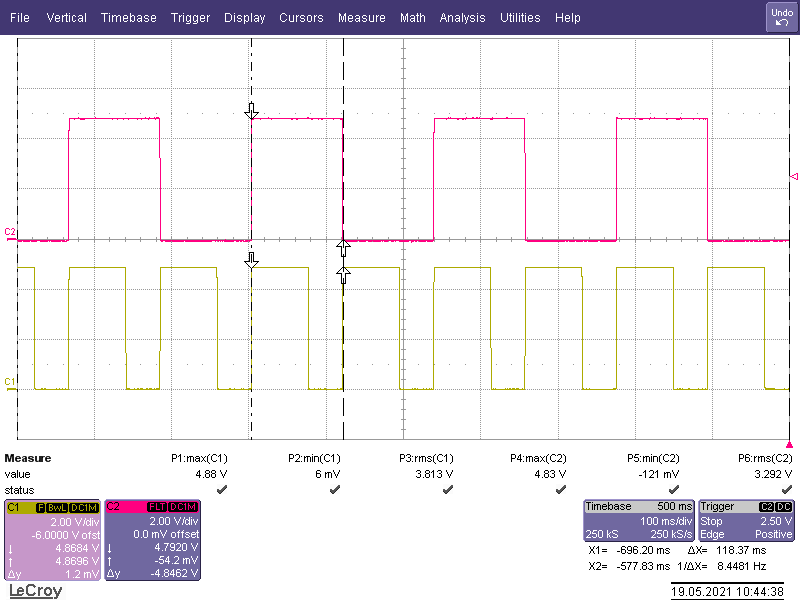
\includegraphics[width=8cm]{Bilder/Systemtakte.png}
        \caption{Teilung des NE555-Takt}
    \end{minipage}
\end{figure}



%%%%%%%%%%%%%%%%%%%%%%%%%%%%%%%%%%%%%%%%%%%%%%%%%%%%%%%%%%%%%%%%%%%%%%%%%%%%%%%%%%%%%%%%%%%%%%%%%%%%%%%%%%%%%%%%%%%%%%%%%																																				%
%														Taktgeber       												%
%																														%
%%%%%%%%%%%%%%%%%%%%%%%%%%%%%%%%%%%%%%%%%%%%%%%%%%%%%%%%%%%%%%%%%%%%%%%%%%%%%%%%%%%%%%%%%%%%%%%%%%%%%%%%%%%%%%%%%%%%%%%%%

\newpage
\subsection{DEZ-Zähler}

%%%%%%%%%%%%%%%%%%%%%%%%%%%%%%%%%%%%%%%%%%%%%%%%%%%%%%%%%%%%%%%%%%%%%%%%%%%%%%%
%																			  %
%								Vorgaben									  %
%																			  %
%%%%%%%%%%%%%%%%%%%%%%%%%%%%%%%%%%%%%%%%%%%%%%%%%%%%%%%%%%%%%%%%%%%%%%%%%%%%%%%

\begin{itemize}
	\item{Wenn die LED D2 (Grün) leuchtet, kann durch Betätigung von SW1 (START)\\ der Messvorgang gestartet werden. Dies macht sich durch das Lauflicht (bestehend aus D39, D40, D41, D42) bemerkbar.}
	
	\item{Nach einer Zeit von ca. 3,6s (Messbar durch Impulszeit von TP20) soll das ganze System durch Betätigung von SW1 erneut gestartet werden können.}
	
	\item{Im Einschaltmoment soll ein verspäteter Nadelimpuls für das korrekte Setzen(default-states) der Schaltung am TP23 gemessen werden können.}
	
	 \item{Leuchtet die LED D1 (Rot), so soll ein Starten der Messung durch Betätigung von SW1 (START) nicht möglich sein.}
\end{itemize}

%%%%%%%%%%%%%%%%%%%%%%%%%%%%%%%%%%%%%%%%%%%%%%%%%%%%%%%%%%%%%%%%%%%%%%%%%%%%%%%
%																			  %
%								Tabelle  									  %
%																			  %
%%%%%%%%%%%%%%%%%%%%%%%%%%%%%%%%%%%%%%%%%%%%%%%%%%%%%%%%%%%%%%%%%%%%%%%%%%%%%%%

\renewcommand{\arraystretch}{2}
\begin{tabularx}{\textwidth}{p{0.2\textwidth}| p{0.6\textwidth} | p{0.05\textwidth} | p{0.1\textwidth}}

 &  & i.o & n.i.o \\

\hline

Stromaufnahme & $I_{G}$: \textcolor{blue}{7,2mA} 					& [x] & [ ] \\

\hline

\multirow{2}{*}{Start Messung}
		& LED D2 und SW1 -> Messung Startet		 					& [x] & [ ] \\
		& $t_{Testzeit}$:	\textcolor{blue}{3,48s}					& [x] & [ ] \\

\hline

\multirow{2}{*}{Nadelimpuls}
		& $t_{Delay}$: \textcolor{blue}{766us}						&[x] & [ ] 	\\
		& $t_{i}$: 	\textcolor{blue}{500us}							&[x] & [ ] 	\\
		
\hline

Tastensperre & LED D1 und SW1 -> Messung Startet nicht 				&[x] & [ ] \\
		
\end{tabularx}
\renewcommand{\arraystretch}{1}

\begin{figure}[htb]
    \centering
    \begin{minipage}[t]{0.45\linewidth}
        \centering
        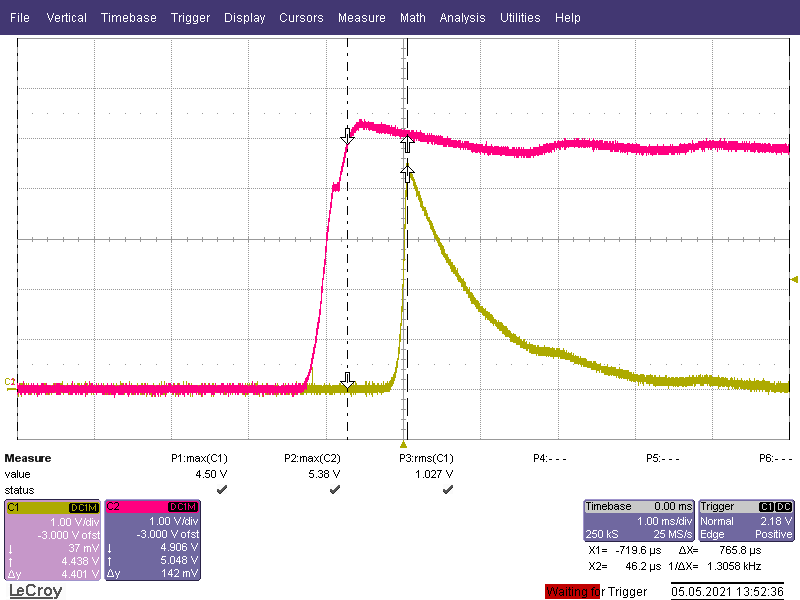
\includegraphics[width=8cm]{Bilder/Resetimpuls.png}
        \caption{Resetimpuls im Einschaltmoment}
    \end{minipage}% <- sonst wird hier ein Leerzeichen eingefügt
    \hfill
    \begin{minipage}[t]{0.45\linewidth}
        \centering
        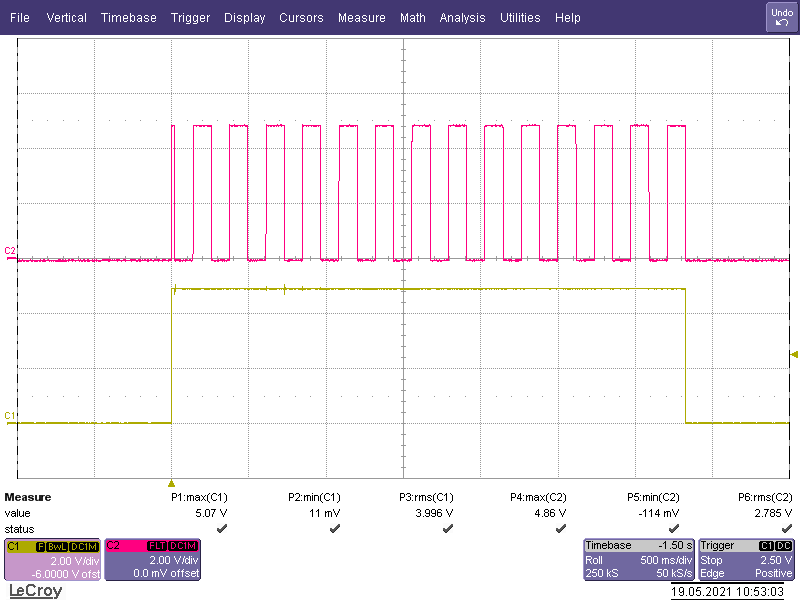
\includegraphics[width=8cm]{Bilder/4Bittakt.png}
        \caption{Taktimpulse nach Starten der Messung}
    \end{minipage} 
\end{figure}

%%%%%%%%%%%%%%%%%%%%%%%%%%%%%%%%%%%%%%%%%%%%%%%%%%%%%%%%%%%%%%%%%%%%%%%%%%%%%%%%%%%%%%%%%%%%%%%%%%%%%%%%%%%%%%%%%%%%%%%%%																																				%
%														Taktgeber       												%
%																														%
%%%%%%%%%%%%%%%%%%%%%%%%%%%%%%%%%%%%%%%%%%%%%%%%%%%%%%%%%%%%%%%%%%%%%%%%%%%%%%%%%%%%%%%%%%%%%%%%%%%%%%%%%%%%%%%%%%%%%%%%%

\newpage
\subsection{Leitungstreiber und Umschaltung}

%%%%%%%%%%%%%%%%%%%%%%%%%%%%%%%%%%%%%%%%%%%%%%%%%%%%%%%%%%%%%%%%%%%%%%%%%%%%%%%
%																			  %
%								Vorgaben									  %
%																			  %
%%%%%%%%%%%%%%%%%%%%%%%%%%%%%%%%%%%%%%%%%%%%%%%%%%%%%%%%%%%%%%%%%%%%%%%%%%%%%%%

\begin{itemize}
	\item{Bei einem High-Signal an TP10 muss das 5V Potenzial auf den Pin 1 von J6 durchgeschaltet werden. Diese Messung muss mit einem Oszilloskop erfolgen, um Pegelschwankungen eindeutig erkennen zu können.}
	
	\item{Nach der Hälfte des High-Signals an TP10 muss auch ein High-Signal an TP11 gemessen werden können.}
	
	\item{Um die Funktion des Analogschalters bestätigen zu können, muss bei gestecktem Jumper (J6) ein 5V Signal für $\dfrac{t_{TP10}}{2}$ an TP5 und TP32 anliegen.}
\end{itemize}

%%%%%%%%%%%%%%%%%%%%%%%%%%%%%%%%%%%%%%%%%%%%%%%%%%%%%%%%%%%%%%%%%%%%%%%%%%%%%%%
%																			  %
%								Tabelle  									  %
%																			  %
%%%%%%%%%%%%%%%%%%%%%%%%%%%%%%%%%%%%%%%%%%%%%%%%%%%%%%%%%%%%%%%%%%%%%%%%%%%%%%%

\renewcommand{\arraystretch}{2}
\begin{tabularx}{\textwidth}{p{0.2\textwidth}| p{0.6\textwidth} | p{0.05\textwidth} | p{0.1\textwidth}}

 &  & i.o & n.i.o \\

\hline

Stromaufnahme & $I_{G}$: \textcolor{blue}{7,6mA} & [x] & [ ] \\

\hline

\multirow{2}{*}{Messspannung}
		& $t_{TP10}$:\textcolor{blue}{228ms}					& [x] & [ ] \\
		& $U_{J6}$: \textcolor{blue}{4,91V}						& [x] & [ ] \\

\hline

\multirow{2}{*}{Umschaltsignal}
		& $t_{delay-TP11}$	\textcolor{blue}{108ms} 				& [x] & [ ] \\
		& $t_{TP11}$: \textcolor{blue}{120ms}						& [x] & [ ] \\

\hline

Umschaltung & Umschaltung von U38A:	& [x] & [ ] \\
		
\end{tabularx}
\renewcommand{\arraystretch}{1}

\begin{figure}[htb]
    \centering
    \begin{minipage}[t]{0.45\linewidth}
        \centering
        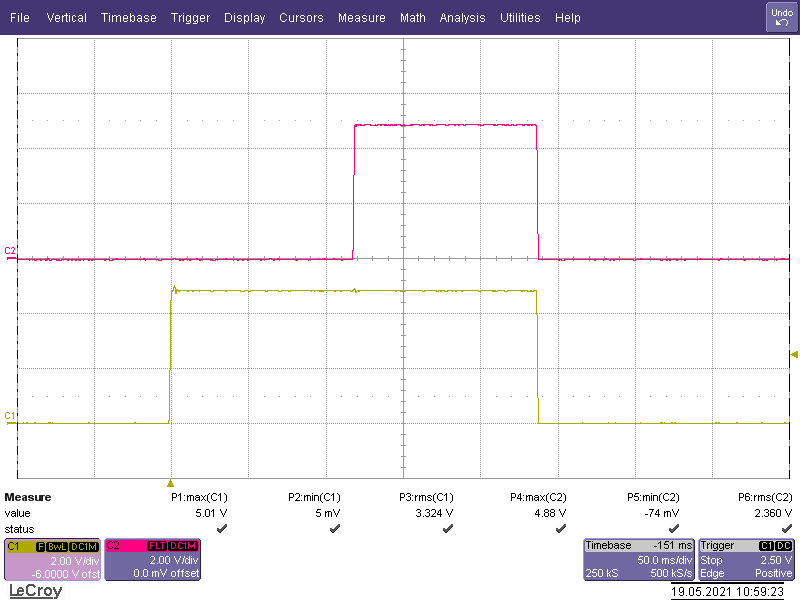
\includegraphics[width=8cm]{Bilder/ASwitch-Umschaltung.png}
        \caption{Umschaltimpuls zwischen den beiden Messungen}
    \end{minipage}% <- sonst wird hier ein Leerzeichen eingefügt
\end{figure}

%%%%%%%%%%%%%%%%%%%%%%%%%%%%%%%%%%%%%%%%%%%%%%%%%%%%%%%%%%%%%%%%%%%%%%%%%%%%%%%%%%%%%%%%%%%%%%%%%%%%%%%%%%%%%%%%%%%%%%%%%																																				%
%														Taktgeber       												%
%																														%
%%%%%%%%%%%%%%%%%%%%%%%%%%%%%%%%%%%%%%%%%%%%%%%%%%%%%%%%%%%%%%%%%%%%%%%%%%%%%%%%%%%%%%%%%%%%%%%%%%%%%%%%%%%%%%%%%%%%%%%%%

\newpage
\subsection{Durchgangsprüfung und Kurzschlussmessung}

%%%%%%%%%%%%%%%%%%%%%%%%%%%%%%%%%%%%%%%%%%%%%%%%%%%%%%%%%%%%%%%%%%%%%%%%%%%%%%%
%																			  %
%								Vorgaben									  %
%																			  %
%%%%%%%%%%%%%%%%%%%%%%%%%%%%%%%%%%%%%%%%%%%%%%%%%%%%%%%%%%%%%%%%%%%%%%%%%%%%%%%

\begin{itemize}
	\item{Analyse des Reset-Impulses, welcher die Schaltung in einen einheitlichen Startzustand bringt.}
	
	\item{Überprüfung der Nadelimpulsunterdrückung durch gleichzeitiges messen an TP32 und Pin 6 von U30.}
\end{itemize}

%%%%%%%%%%%%%%%%%%%%%%%%%%%%%%%%%%%%%%%%%%%%%%%%%%%%%%%%%%%%%%%%%%%%%%%%%%%%%%%
%																			  %
%								Tabelle  									  %
%																			  %
%%%%%%%%%%%%%%%%%%%%%%%%%%%%%%%%%%%%%%%%%%%%%%%%%%%%%%%%%%%%%%%%%%%%%%%%%%%%%%%

\renewcommand{\arraystretch}{2}
\begin{tabularx}{\textwidth}{p{0.2\textwidth}| p{0.6\textwidth} | p{0.05\textwidth} | p{0.1\textwidth}}

 &  & i.o & n.i.o \\

\hline

Stromaufnahme & $I_{G}$: \textcolor{blue}{7,7mA} 					& [x] & [ ] \\

\hline

Reset-Impuls & $t_{RST}$: \textcolor{blue}{20ns} 					& [x] & [ ] \\

\hline

\multirow{2}{*}{Nadel-Impuls}
		& $t_{TP32_{Nadel-Impuls}}$: \textcolor{blue}{305ns}	 	& [x] & [ ] \\
		& $U_{Pin6 U30_{Nadel-Impuls}}$: \textcolor{blue}{0V}		& [x] & [ ] \\
		
\end{tabularx}
\renewcommand{\arraystretch}{1}

\begin{figure}[htb]
    \centering
    \begin{minipage}[t]{0.45\linewidth}
        \centering
        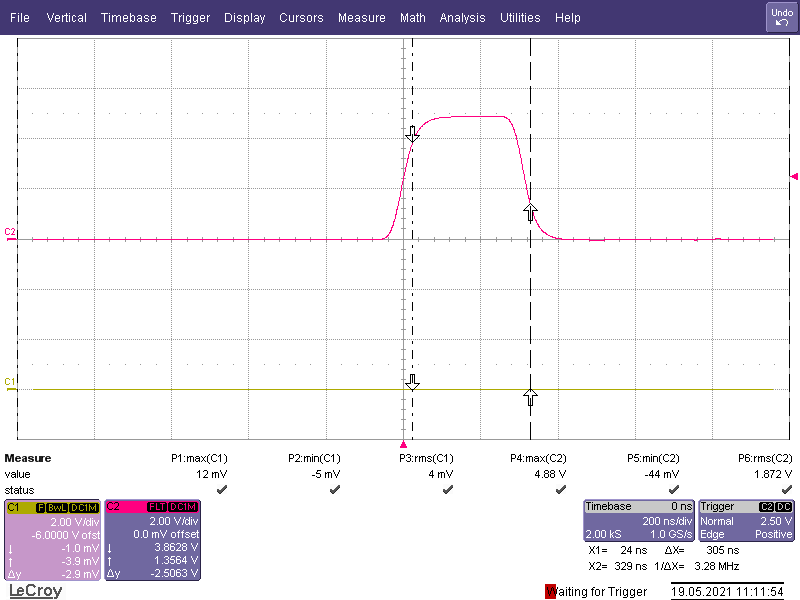
\includegraphics[width=8cm]{Bilder/Fehlerimpuls.png}
        \caption{Unterdrückung eines Set-Impuls im Fehlerfall. }
    \end{minipage}% <- sonst wird hier ein Leerzeichen eingefügt
    \hfill
    \begin{minipage}[t]{0.45\linewidth}
        \centering
        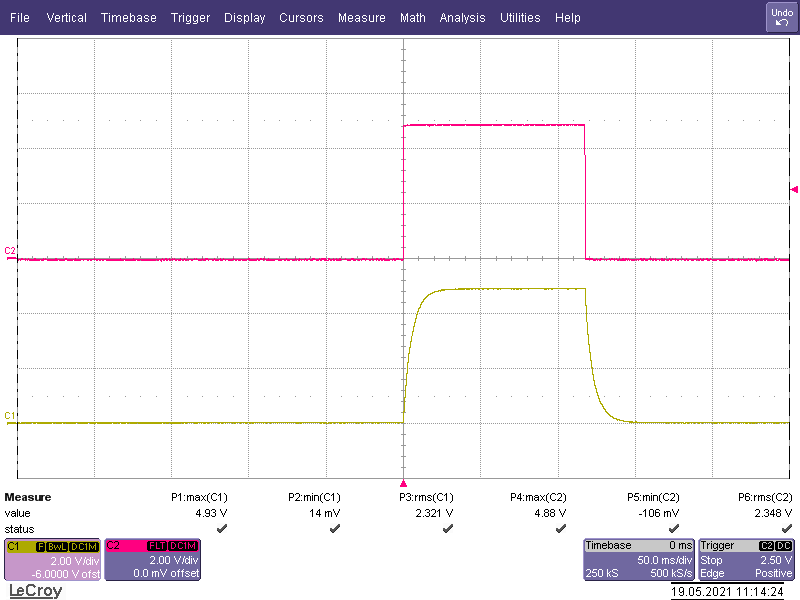
\includegraphics[width=8cm]{Bilder/LowpassFilter.png}
        \caption{Set-Impuls bei fehlerfreier Leitung}
    \end{minipage} 
\end{figure}

%%%%%%%%%%%%%%%%%%%%%%%%%%%%%%%%%%%%%%%%%%%%%%%%%%%%%%%%%%%%%%%%%%%%%%%%%%%%%%%%%%%%%%%%%%%%%%%%%%%%%%%%%%%%%%%%%%%%%%%%%																																				%
%														Taktgeber       												%
%																														%
%%%%%%%%%%%%%%%%%%%%%%%%%%%%%%%%%%%%%%%%%%%%%%%%%%%%%%%%%%%%%%%%%%%%%%%%%%%%%%%%%%%%%%%%%%%%%%%%%%%%%%%%%%%%%%%%%%%%%%%%%

\newpage
\subsection{Konstantstrommessung}

%%%%%%%%%%%%%%%%%%%%%%%%%%%%%%%%%%%%%%%%%%%%%%%%%%%%%%%%%%%%%%%%%%%%%%%%%%%%%%%
%																			  %
%								Vorgaben									  %
%																			  %
%%%%%%%%%%%%%%%%%%%%%%%%%%%%%%%%%%%%%%%%%%%%%%%%%%%%%%%%%%%%%%%%%%%%%%%%%%%%%%%

\begin{itemize}
	\item{Funktion der Konstantstromquelle prüfen durch Stecken eines Jumpers auf J6 und Starten eines Messvorganges. Wenn RV2 und RV3 in Mittelstellung sind, dann ist an TP 6 ein High-Impuls zu erwarten.}
	
	\item{Prüfen, ob die richtigen Takte bzw. Steuersignale an dem Schieberegister anliegen.}
	
	\item{Prüftabelle mit verschiedenen Kabelwiderständen und den dazugehörigen rechnerischen Werten anlegen.}
\end{itemize}

%%%%%%%%%%%%%%%%%%%%%%%%%%%%%%%%%%%%%%%%%%%%%%%%%%%%%%%%%%%%%%%%%%%%%%%%%%%%%%%
%																			  %
%								Tabelle  									  %
%																			  %
%%%%%%%%%%%%%%%%%%%%%%%%%%%%%%%%%%%%%%%%%%%%%%%%%%%%%%%%%%%%%%%%%%%%%%%%%%%%%%%

\renewcommand{\arraystretch}{2}
\begin{tabularx}{\textwidth}{p{0.25\textwidth}| p{0.55\textwidth} | p{0.05\textwidth} | p{0.1\textwidth}}

 &  & i.o & n.i.o \\

\hline

Stromaufnahme & $I_{G}$: \textcolor{blue}{7,9mA} & [x] & [ ] \\

\hline

Konstantstromquelle & Funktion der Konstantstromquelle: 	& [ ] & [x] \\

\hline

Schieberegister Takte & Funktion der Steuersignale: 		& [ ] & [x] \\
		
\end{tabularx}
\renewcommand{\arraystretch}{1}

\vspace{1,5cm}
\textbf{Bemerkung:}
\\
Die Inbetriebnahme dieses Schaltungsteiles hat auf Grund von verschiedenen Fehler einen größeren Zeitraum als geplant eingenommen. Im Kapitel Fehleranalyse wird zwar auf die Fehler und deren Behebung eingegangen, aus zeitlichen Gründen ist dieser Teil aber kein offizieller Teil meines betrieblichen Auftrages.


\begin{figure}[htb]
    \centering
    \begin{minipage}[t]{0.45\linewidth}
        \centering
        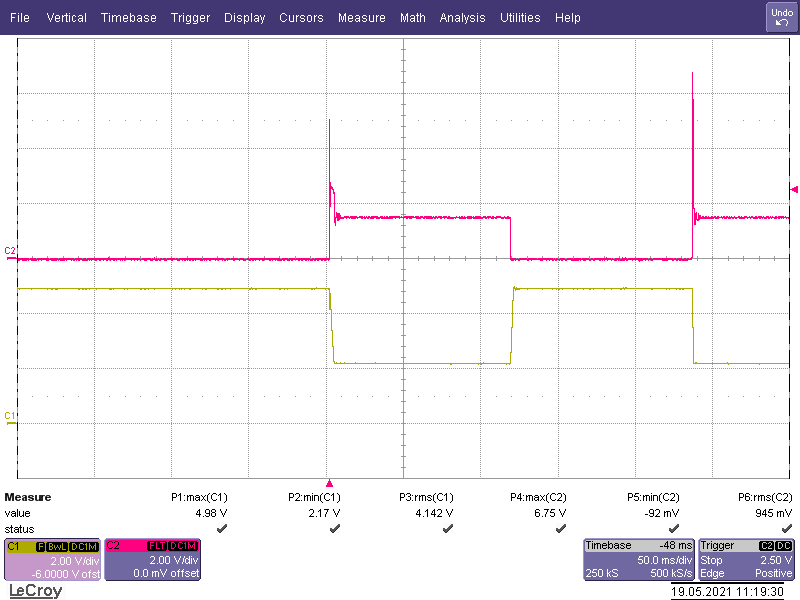
\includegraphics[width=8cm]{Bilder/INA-Spannung.png}
        \caption{CH2 = Spannung nach dem INA (Strommessung)\\
        			CH1 = Regelung des Stromes über die Gate-Source-Spannung}
    \end{minipage}% <- sonst wird hier ein Leerzeichen eingefügt
    \hfill
    \begin{minipage}[t]{0.45\linewidth}
        \centering
        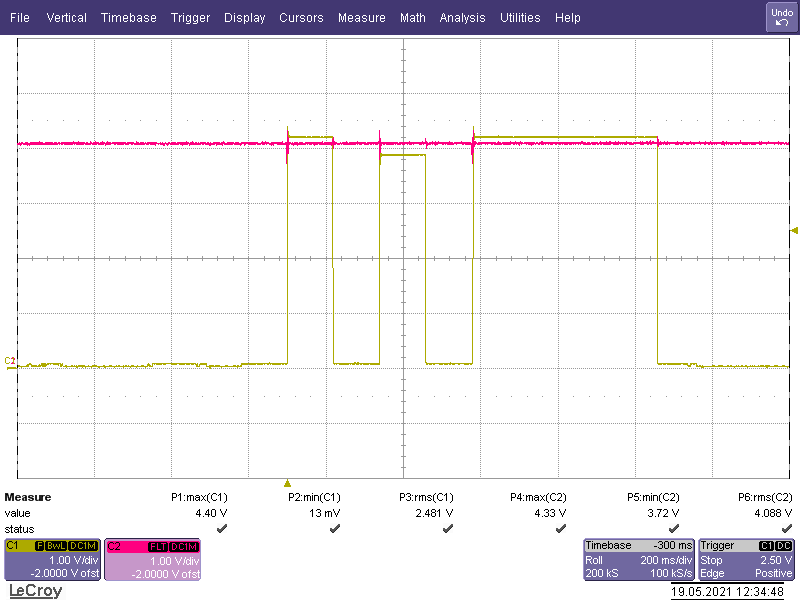
\includegraphics[width=8cm]{Bilder/Auswertung-Widerstand.png}
        \caption{CH2 = Grenzwiderstand (Referenzspannung)\\ 
        			CH1 = Indirekte Widerstandswerte (Spannung über Q1)}
    \end{minipage} 
\end{figure}

Die Abbildung 12 zeigt eine Konstantstrommessung mit 0R, 10R und einem Kurzschluss (von links nach rechts). 


\newpage
\section{Fehleranalyse}

\begin{center}
In diesem Kapitel werden die Fehler, welche bei der Inbetriebnahme aufgedeckt wurden behandelt. Der sich im Anhang befindenden Schaltplan \glqq Abschlussprojekt Kabeltester  V-01\grqq{} vermerkt diese mit der Beschriftung \glqq Fehler 1-5\grqq{}. Schaltungsdesignefehler wurden mit Fädeldraht verbessert.  
\end{center}



\subsection{Fehler 1}

Bei dem ersten Fehler handelt es sich um ein Footprintfehler. Der Sicherung F1 wurde im Schaltungsteil \glqq Versorgung \grqq{} auf Seite 2, ein Falsches Footprint zugewiesen. Somit ist es nicht möglich den Sicherungssockel zu verlöten. 


\subsection{Fehler 2}

Im Schaltungsteil \glqq NE555 Taktgeber \grqq{} auf Seite 3, wurde im Abschnitt \glqq Taktteilung \grqq{} das IC U8A (Inverter) verpolt. Durch anheben der Pin's 3 und 4 wurde mit der Hilfe von Fädeldraht dieser Fehler behoben.



\subsection{Fehler 3}

Bei der Inbetriebnahme der Konstantstromquelle auf Seite 7 stellte sich heraus, dass die Schaltung in dieser Konstellation zum schwingen beginnt. Durch einen Mitarbeiter der Entwicklung wurde ich auf einen fehlenden Widerstand zwischen TP3 und Pin 7 (U19A) hingewiesen. Durch eine fehlerhafte Einstellung des Simulationsprogrammes, konnte ich im Vorfeld den Fehler nicht erkennen. Der durch hohe Frequenzen auftretende Impedanzeinbruch, welcher die Ausgänge U19A Pin 7 und U17A Pin 4 miteinander kurzschließt, wurde mir in früheren Simulationen nicht Angezeigt und von meiner Seite aus nicht bedacht. Zur Fehlerbehebung wurde die Leiterbahn zwischen TP3 und Pin 7 (U19A) aufgetrennt und mit einem 10k Widerstand versehen. 



\subsection{Fehler 4}

Nach Behebung des \glqq Fehler 3 \grqq{} war ein korrektes einstellen des Konstantstromes nicht möglich. Das Problem hierbei liegt in der Versorgung von U19. Bei einem Idealen Leitungswiderstand von 0R liegt an Pin 4 die Versorgungsspannung von U19 an. Intern wird dieses Signal durch einen \glqq Nicht invertierenden Verstärker \grqq{} verstärkt. Da ein OP das Eingangssignal nie auf einen Pegel, größer als seine Betriebsspannung verstärken kann und durch Spannungsabfall am \glqq High und Low - Side Transistor \grqq{} der Ausgangsstufe das verstärkte Signal nicht den Wert der Versorgungsspannung erreichen kann, kommt es zu einer falschen Strommessung. Durch Trennung der Leitung, welche U19 mit +5V versorgt und anschließender Versorgung von U19 mit der Eingangsspannung (+9V) wurde dieses Problem behoben. 

\newpage

\subsection{Fehler 5}

Das zu erwartende Signal an TP36 konnte nicht gemessen werden. Der Schiebeimpuls kam dabei zu früh. Durch invertieren des \glqq System Takt 2 \grqq{} wurde dieser Fehler behoben.



\subsection{Fehler 6}


Wird der Eingang \glqq SRCLR \grqq{} der Schieberegister U20A und U21A mit dem Label \glqq RESET \grqq{} verbunden, so wird die Schaltung dauerhaft zurückgesetzt. 
Wird eine Messung gestartet, so kommt es zu einen positiven Nadelimpuls. Die \glqq Clear-Eingänge \grqq{} der Schieberegister sind dabei Low-Aktiv. 
\\
Durch eine Invertierung des RESET-Impulses oder durch das Verbinden mit +5V kann dieser Fehler behoben oder unterdrückt werden.

\newpage
\documentclass[a4paper,11pt]{scrartcl}

\usepackage[utf8]{inputenc}
\usepackage[ngerman]{babel}
\usepackage[T1]{fontenc}
\usepackage{amsmath}
\usepackage{graphicx}
\usepackage{tabularx}
\usepackage[a4paper, left=2cm, right=2cm, top=2.8cm, bottom=2.8cm]{geometry}
\usepackage{tikz}   
\usepackage[scaled]{helvet}
\usepackage{tabto} 
\usepackage{fancyhdr}
\usepackage{multirow}

\renewcommand*{\familydefault}{\sfdefault}

\pagestyle{fancy}

\setkomafont{section}{\huge}
\setkomafont{subsection}{\Large}


\lhead{Maximilian Hoffmann}
\chead{Betrieblicher Auftrag \\ \textbf{Kabeltester}}
\rhead{
\includegraphics[width=3cm]{Bilder/BMK_LOGO.png}}

\begin{document}

\section{Analyse Leitungswiderstandes}

Ein weiterer Teilbereich dieser Dokumentation, ist die theoretische Analyse des maximal zulässigen Leitungswiderstandes eines Programmierkabels. Dabei wurde mit Hilfe des Simulationsprogramm \glqq LT-Spice\grqq{} ein Ersatzschaltbild eines typischen Programmieraufbaus erstellt.\\

\begin{center}
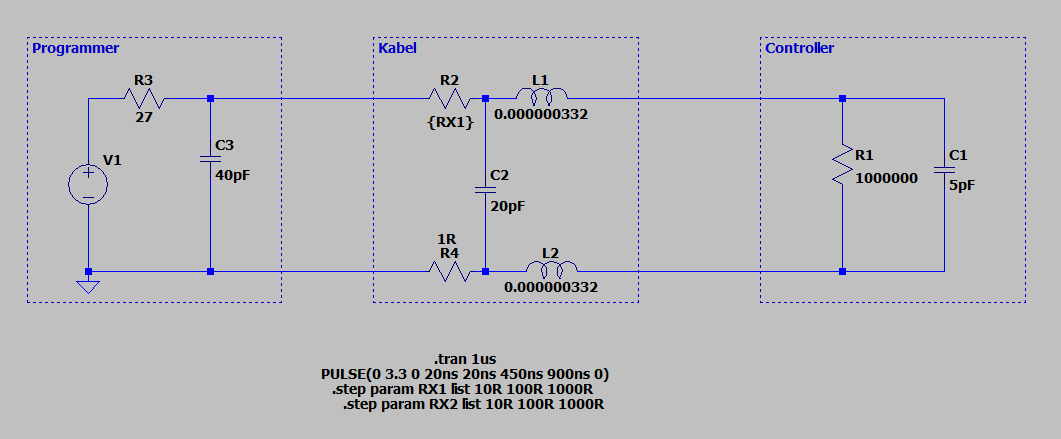
\includegraphics[width=17cm]{Bilder/LTC-SCHALTBILD.png}
\end{center}

Anhand der Datenblätter, welche die Eingangs und Ausgangs Eigenschaften von Controller und Programmer der Firma ST beschreiben, wurden Ersatzschaltbilder erstellt. Die passenden Induktivitäten und Kapazitäten des Programmierkabels wurden mit Hilfe eines Online-Rechner für ein 20cm Kabel berechnet.
\\
\\
Um den Programmiervorgang simulieren zu können gibt die Spannungsquelle V1 ein Rechtecksignal mit ca. 1,1MHz aus. Dies entspricht laut Datenblatt den maximalen Programmiertakt eines ST-Link Programmer. Die zeitliche Dauer einer Signalflanke wurde dabei mit ca.20ns kalkuliert.
\\
\\
Bei der Betrachtung der Signalflanken über Programmer und Controller, mit 10R, 100R und 1000R Leitungswiderstand, wurde mir persönlich nicht sofort klar, warum ein geringer Leitungswiderstand so wichtig für den Programmiervorgang ist. 

\begin{center}
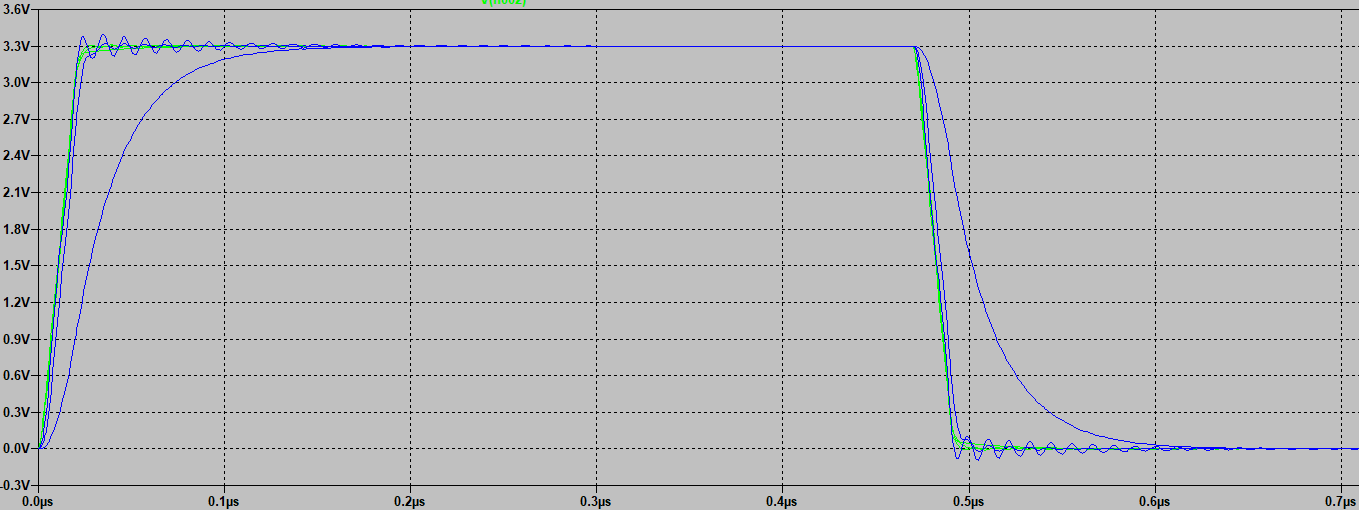
\includegraphics[width=17cm]{Bilder/LTC-SIGNALVERLAUF1.png}
\end{center}

\newpage

Ein differenzielle Messung zwischen Programmer und Controller mit 10R, 100R und 1000R Leitungswiderstand  zeigt den Spannungsunterschied zwischen den beiden Punkten zur selben Zeit. Hierbei zeigt sich, dass während einer Signalflanke kurzzeitig zwischen Programmer und Kontroller einer Potentialunterschied auftritt. Dieser wird mit steigenden Leitungswiderstand größer. Der kleinste Ausbruch tritt bei einem Leitungswiderstand von 10R auf.


\begin{center}
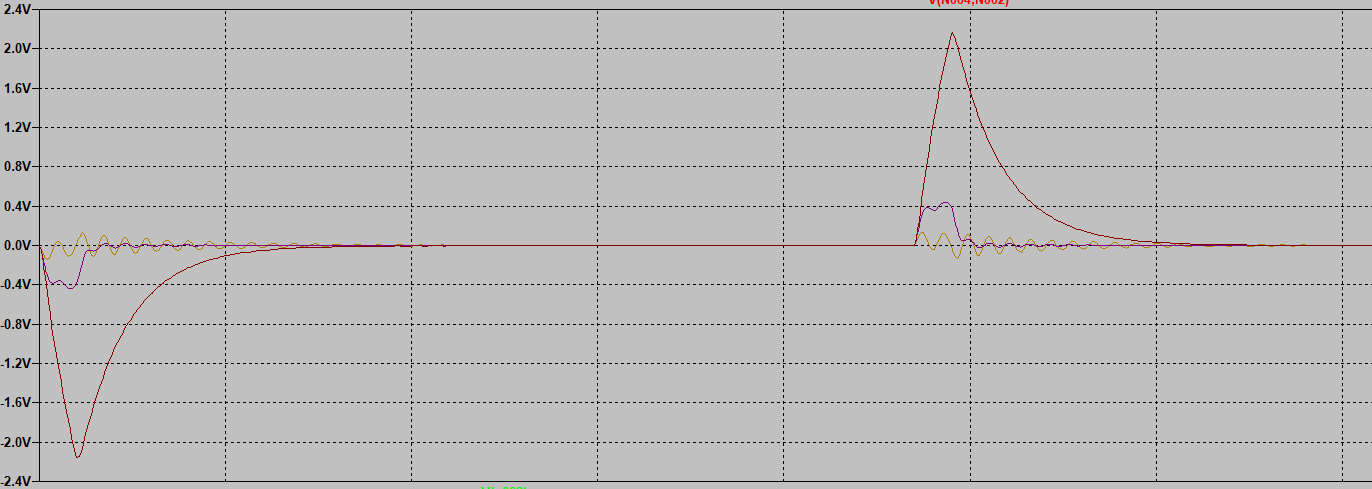
\includegraphics[width=17cm]{Bilder/LTC-SIGNALVERLAUF2.png}
\end{center}

Hierbei handelt es sich um parasitäre Effekte. 
\\
Sie sind unerwünscht und entstehen durch die physikalischen Eigenschaften der Bauelemente. Besonders bei hochfrequenten Anwendungen stellen diese Effekte ein großes Problem dar.
\\
Durch elektrische und magnetische Felder zwischen zwei Punkten, können andere Leitungen gestört werden. Dabei kann es zu Datenübertragungsfehlern kommen.
\\
\\
Aus meiner Simulation geht hervor, das die parasitären Effekte bis zu einem Leitungswiderstand von 10R vernachlässigbar sind. Das von mir entwickelte Prüfgerät wurde daher auf einen Grenzwert von 5R eingestellt. 


\end{document}
\newpage
\input{BA_Stückliste_Stromaufnahme}
\newpage
\section{Anhang}

\begin{itemize}
	\item{Lastenheft}
	
	\item{Pflichtenheft}
	
	\item{Teilauftrag Layout}
	
	\item{Teilauftrag Bestückung}
	
	\item{Blockschaltplan}
	
	\item{Schaltplan}
	
	\item{Layout}
	
	\item{Bestückungsplan}
\end{itemize}


Hallo Hoflloasdfkljasöldfjas





\end{document}